\documentclass{gost}

%-------------------------------------------------------------------------------
%
% ПЕРЕМЕННЫЕ
%
%-------------------------------------------------------------------------------

\newcommand{\universityFullName}{Федеральное государственное бюджетное
образовательное учреждение высшего образования Саратовский Государственный
Технический Университет имени Гагарина Ю.А.}
\newcommand{\universityShortName}{СГТУ им. Гагарина Ю.А.}
\newcommand{\department}{Прикладные информационные технологии}
\newcommand{\nirName}{Лабораторная работа по установке и знакомству с ОС
FreeBSD}
\newcommand{\nirType}{заключительный}
\newcommand{\subject}{Программные и аппаратные технологии умного города}

%-------------------------------------------------------------------------------
%
% ДОКУМЕНТ
%
%-------------------------------------------------------------------------------


\begin{document}
	\gostTitlePage

	\section{Загрузка ОС FreeBSD}
		\begin{figure}[H]
			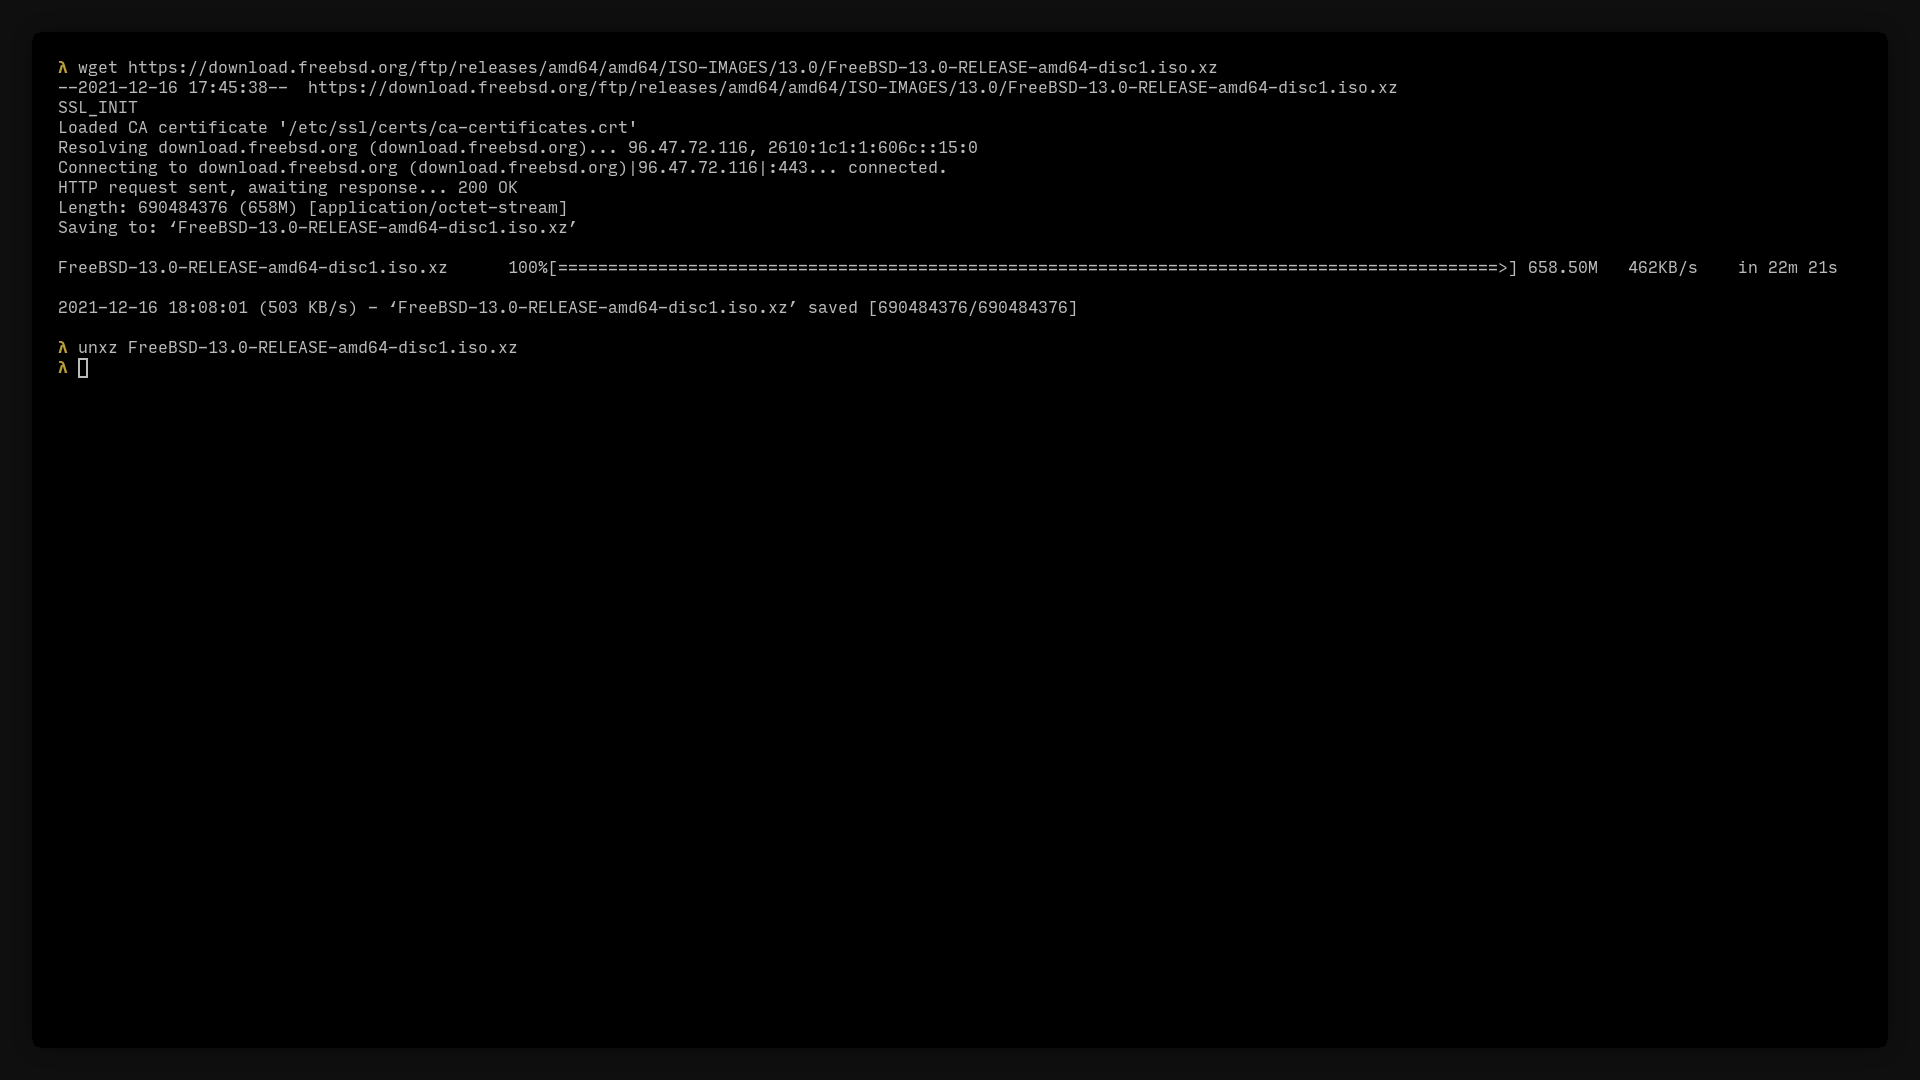
\includegraphics[width=\textwidth,clip=true]{img/1.png}
			\caption{Загрузка ОС FreeBSD}
		\end{figure}

	\section{Настройка виртуальной машины}
		\begin{figure}[H]
			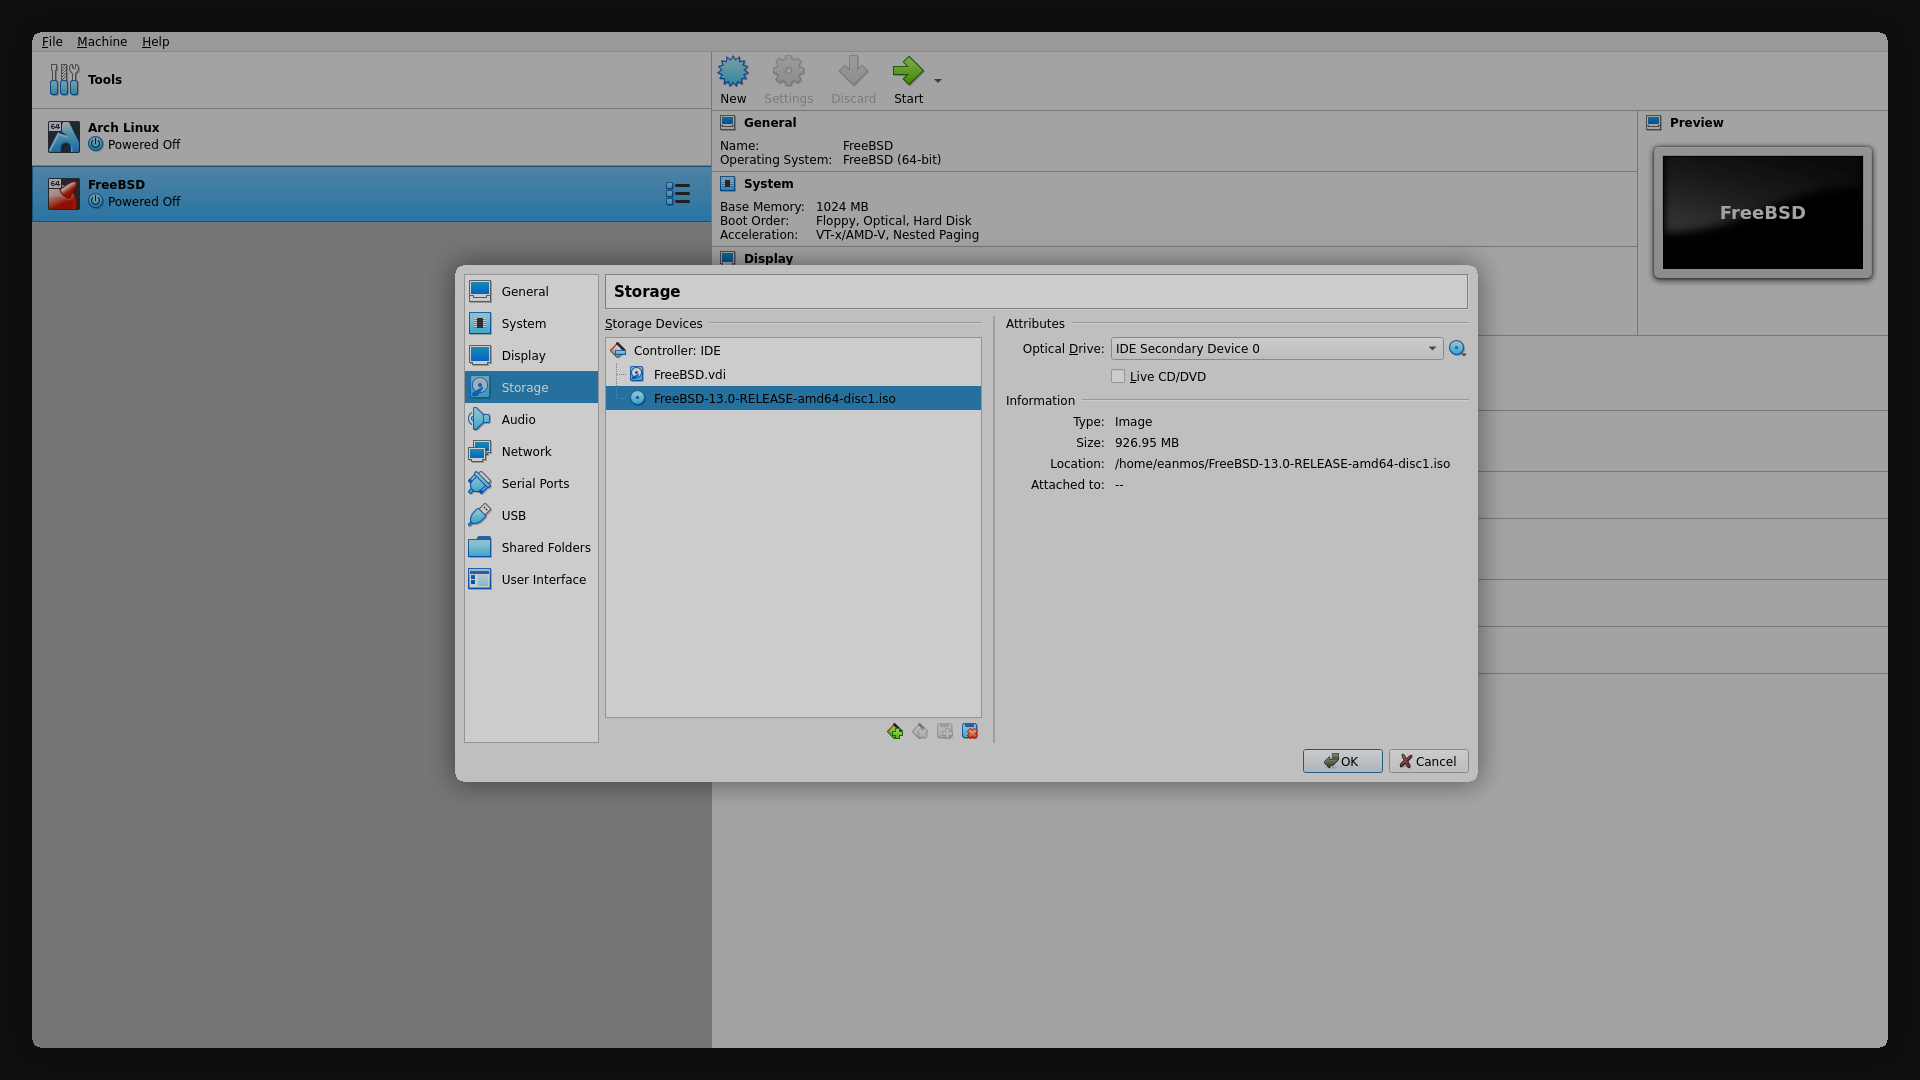
\includegraphics[width=\textwidth,clip=true]{img/2.png}
			\caption{Настраиваем виртуальную машину. Вставляем в CD-ROM виртуальной
			машины ISO-образ с ОС FreeBSD}
		\end{figure}

		\begin{figure}[H]
			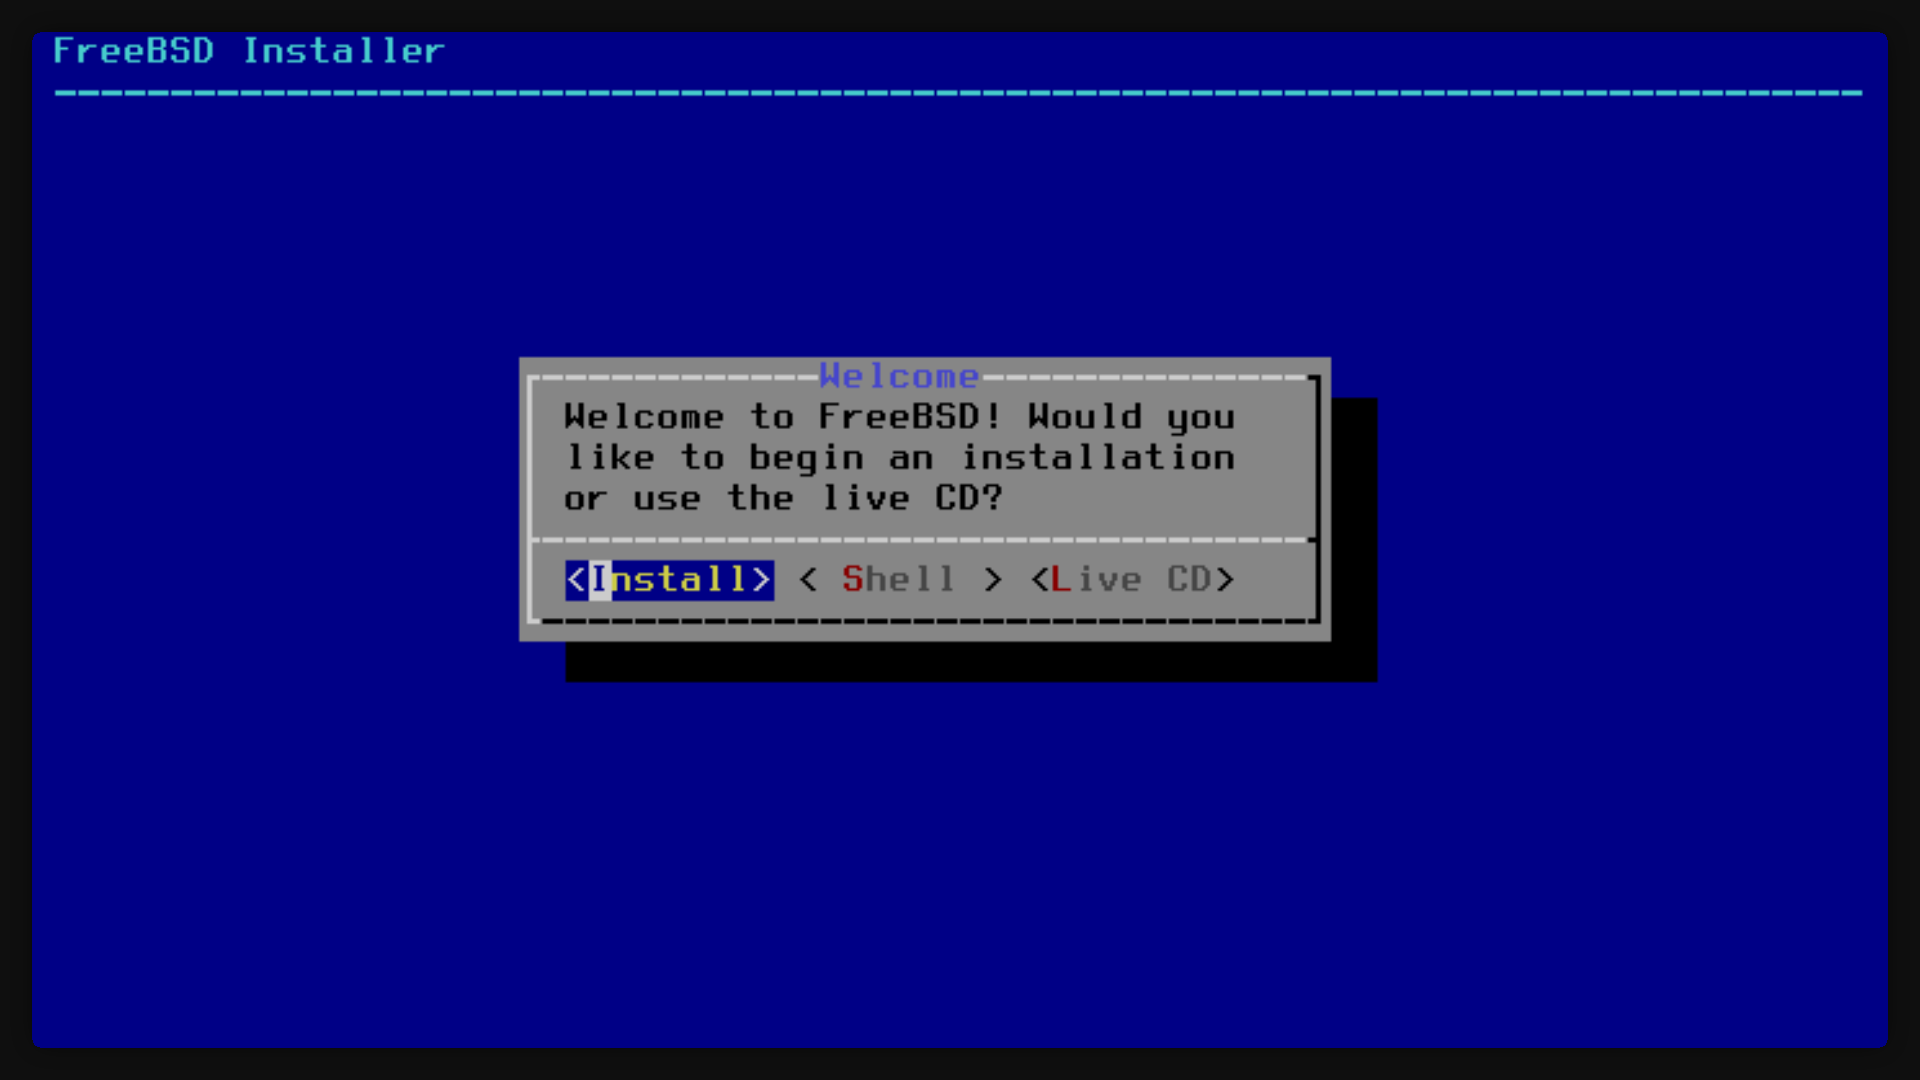
\includegraphics[width=\textwidth,clip=true]{img/3.png}
			\caption{Запускаем виртуальную машину и начинаем процесс установки}
		\end{figure}

	\section{Выбор раскладки клавиатуры}
		\begin{figure}[H]
			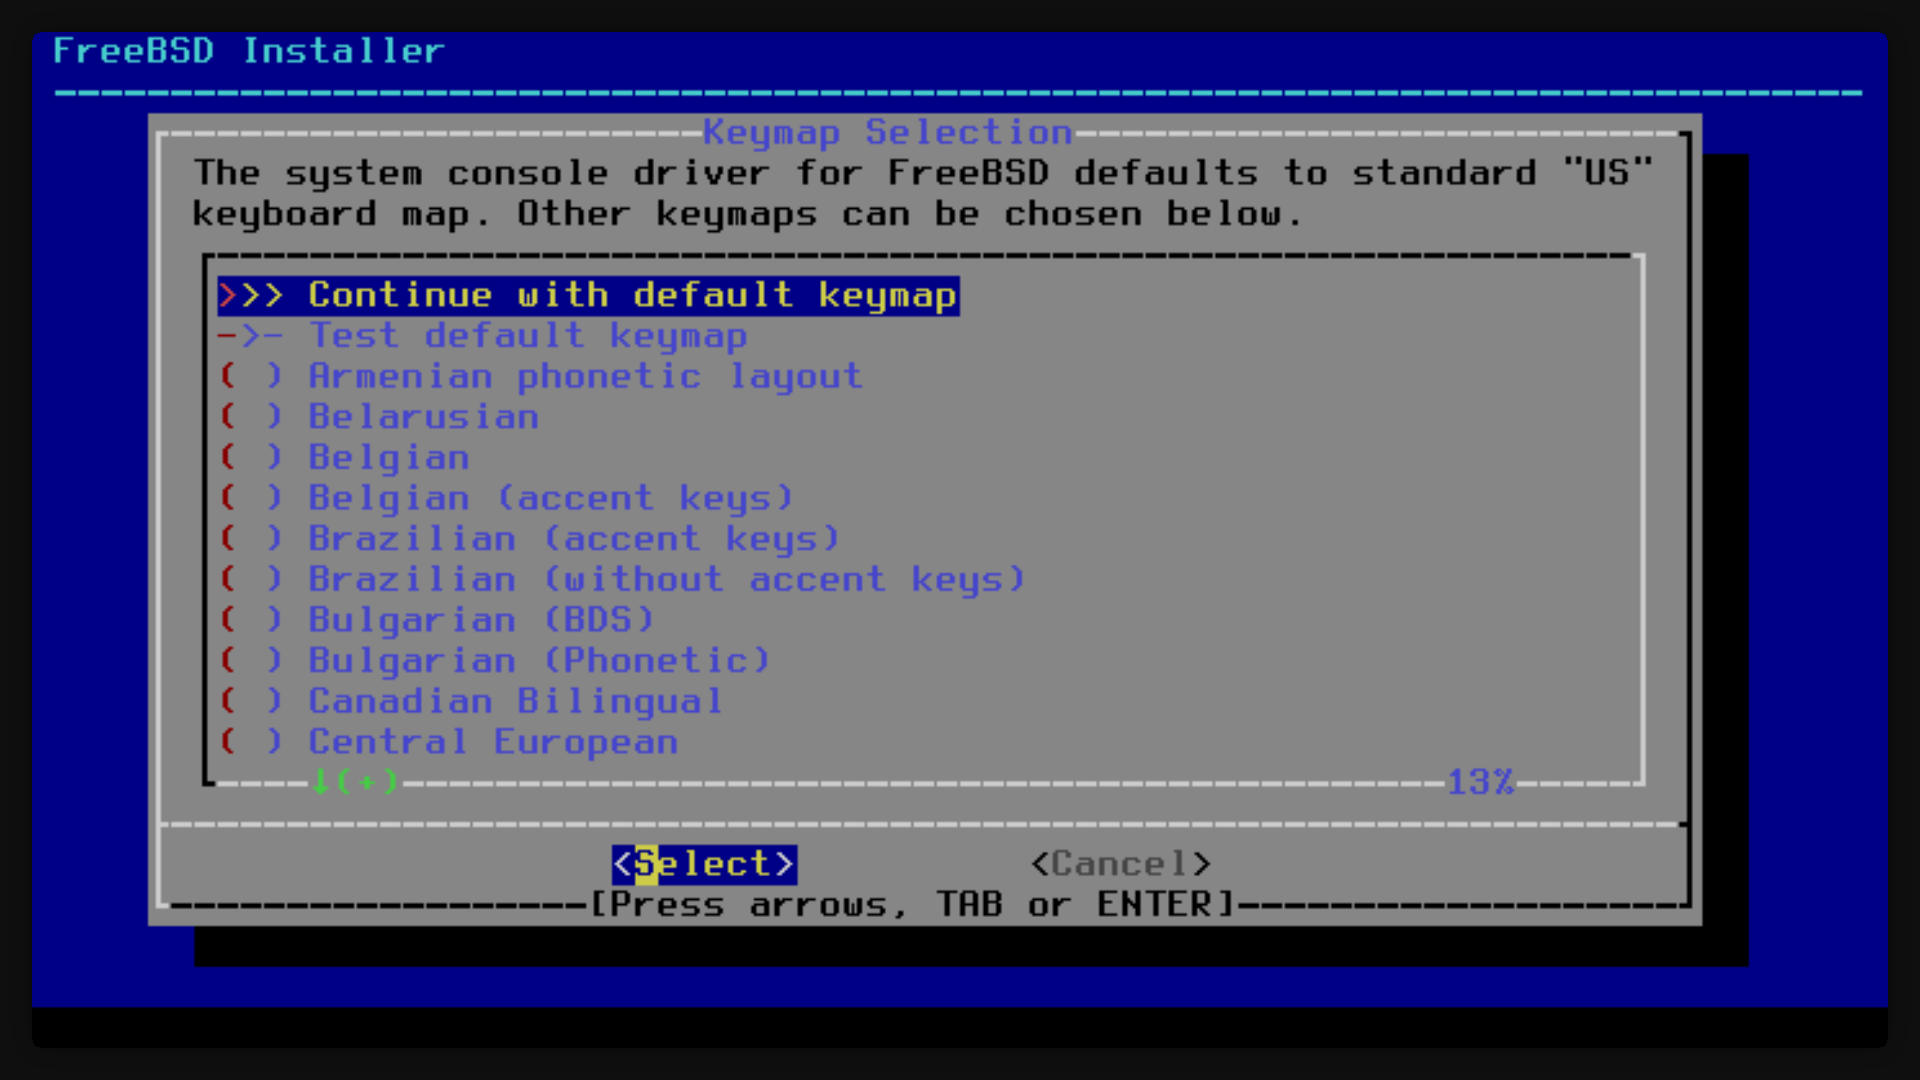
\includegraphics[width=\textwidth,clip=true]{img/4.png}
			\caption{Выбираем стандартную раскладку клавиатуры}
		\end{figure}

	\section{Выбор имени хоста}
		\begin{figure}[H]
			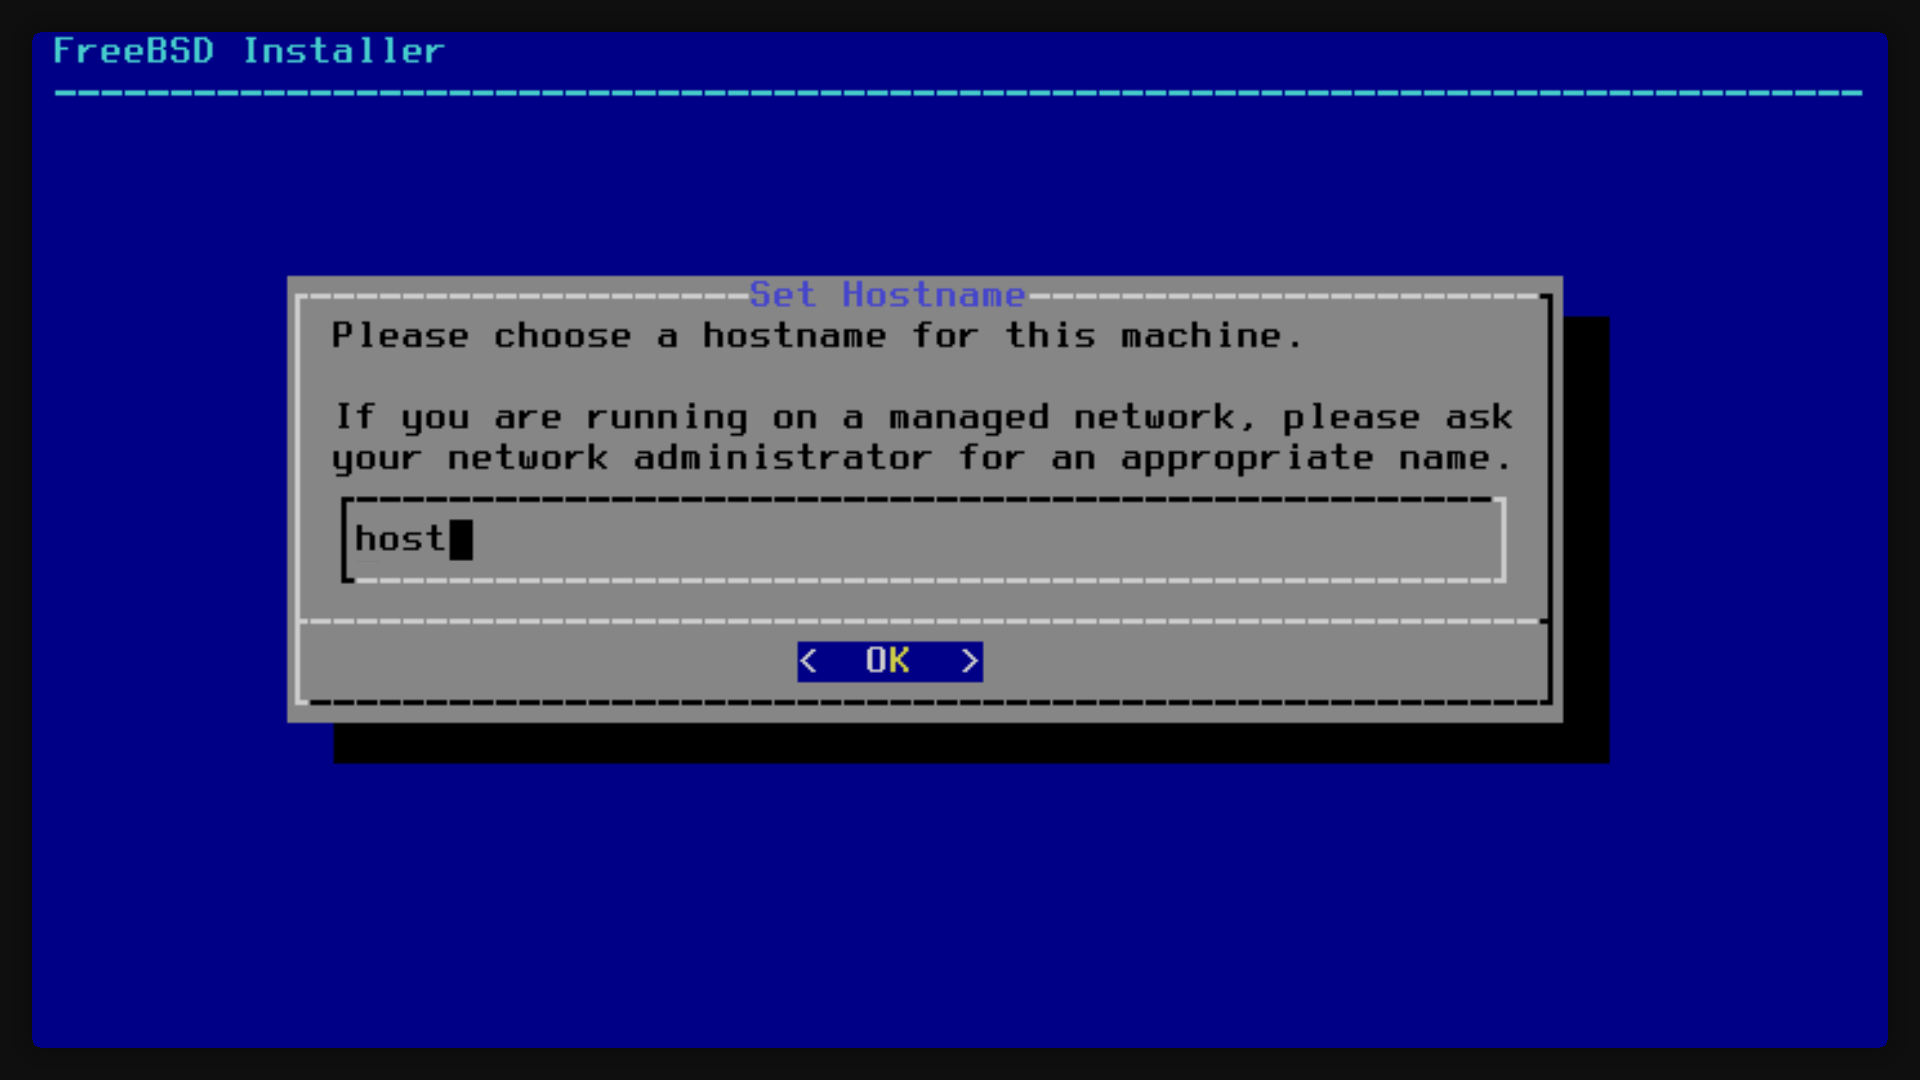
\includegraphics[width=\textwidth,clip=true]{img/5.png}
			\caption{В качестве имени хоста выберем \enquote{host}}
		\end{figure}

	\section{Выбор опциональных компонентов системы}
		\begin{figure}[H]
			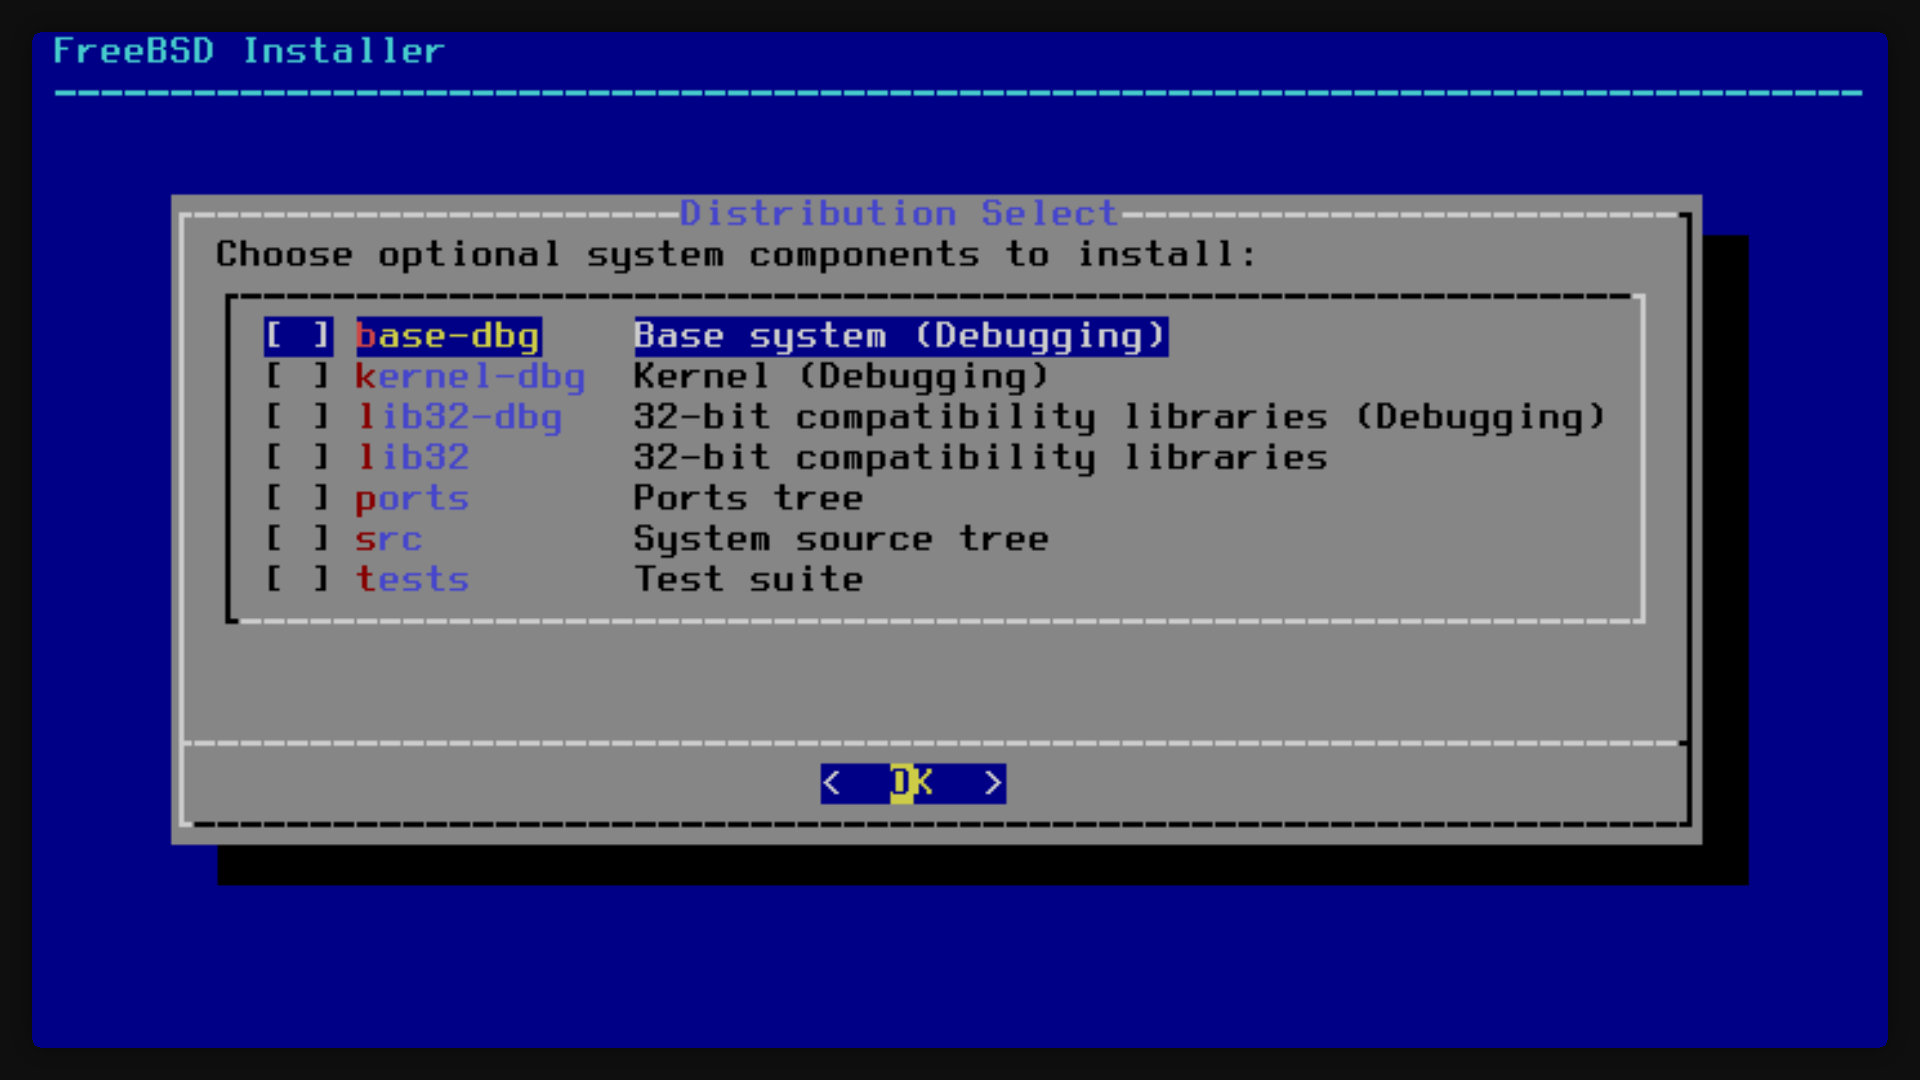
\includegraphics[width=\textwidth,clip=true]{img/6.png}
			\caption{Мы не будем устанавливать никакие опциональные компоненты системы}
		\end{figure}

	\section{Разметка диска для установки}
		\begin{figure}[H]
			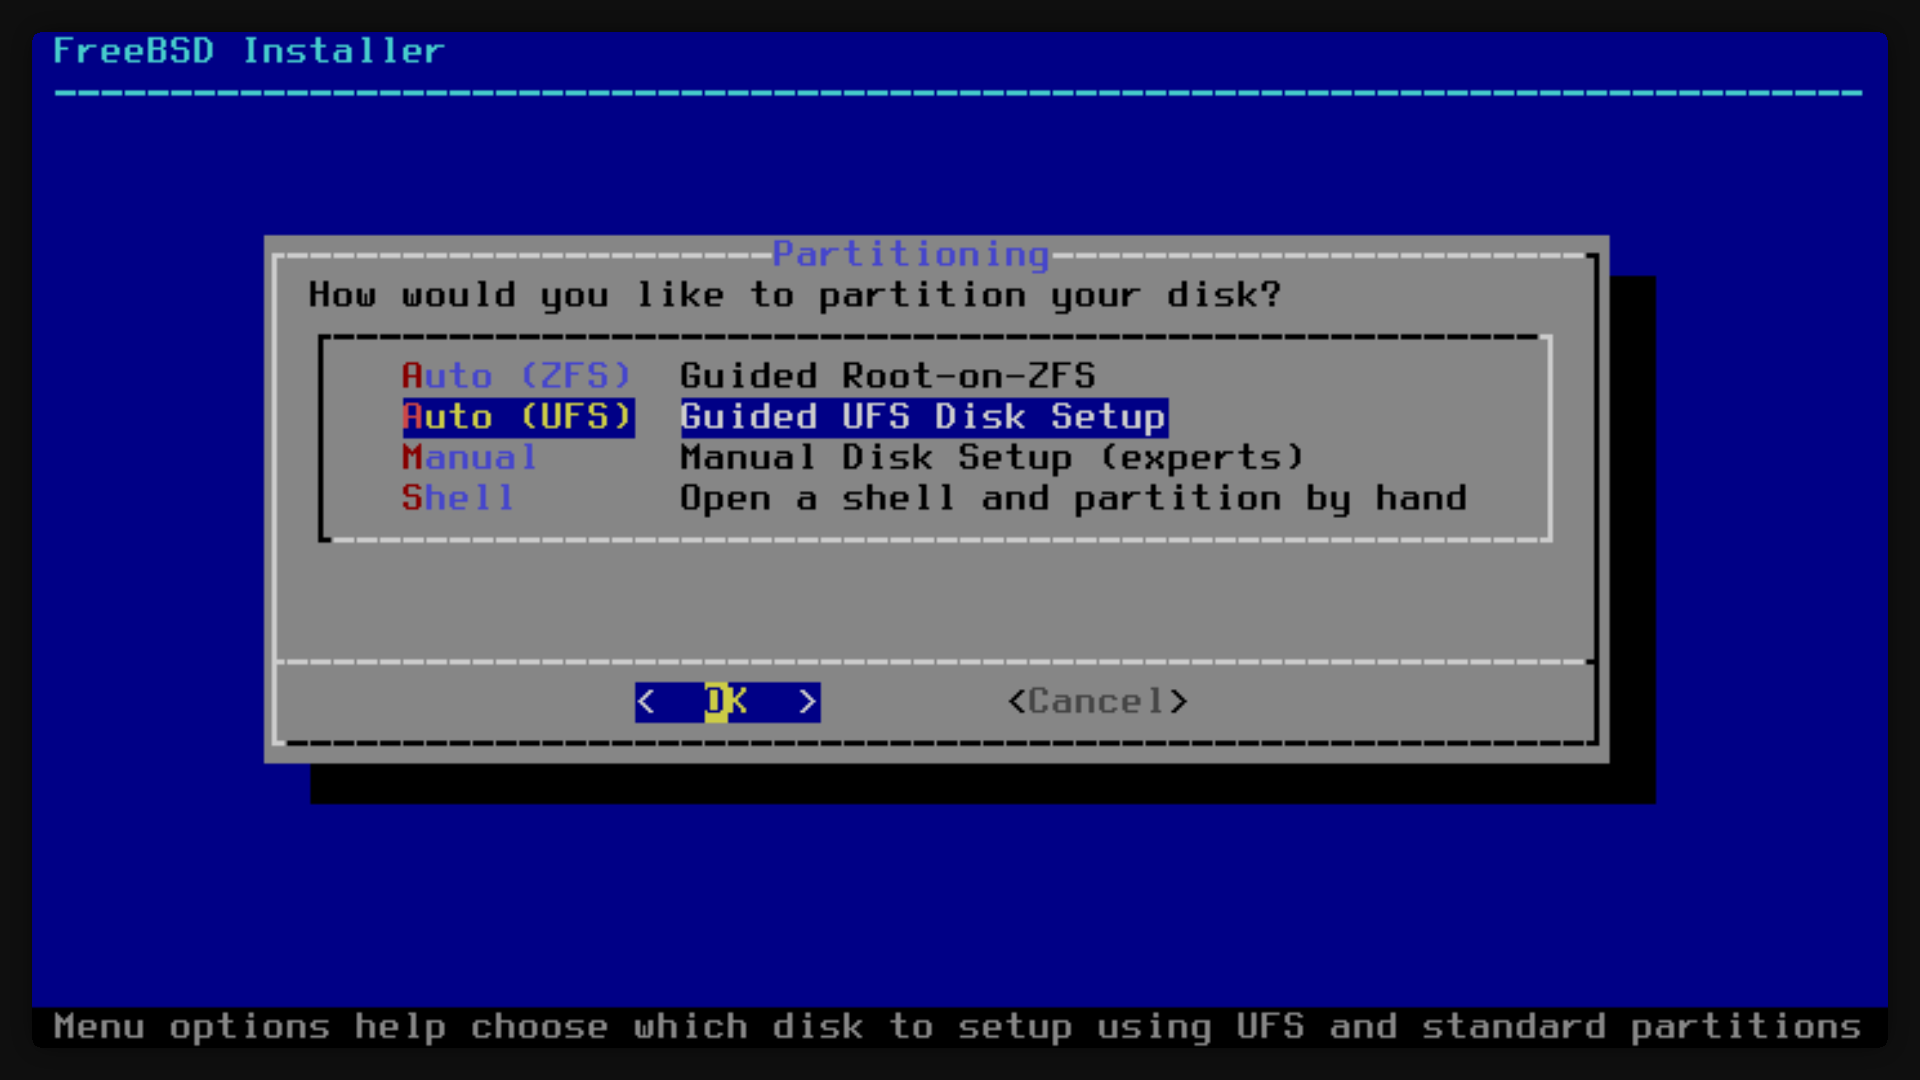
\includegraphics[width=\textwidth,clip=true]{img/7.png}
			\caption{Выбираем автоматическую разметку диска}
		\end{figure}

		\begin{figure}[H]
			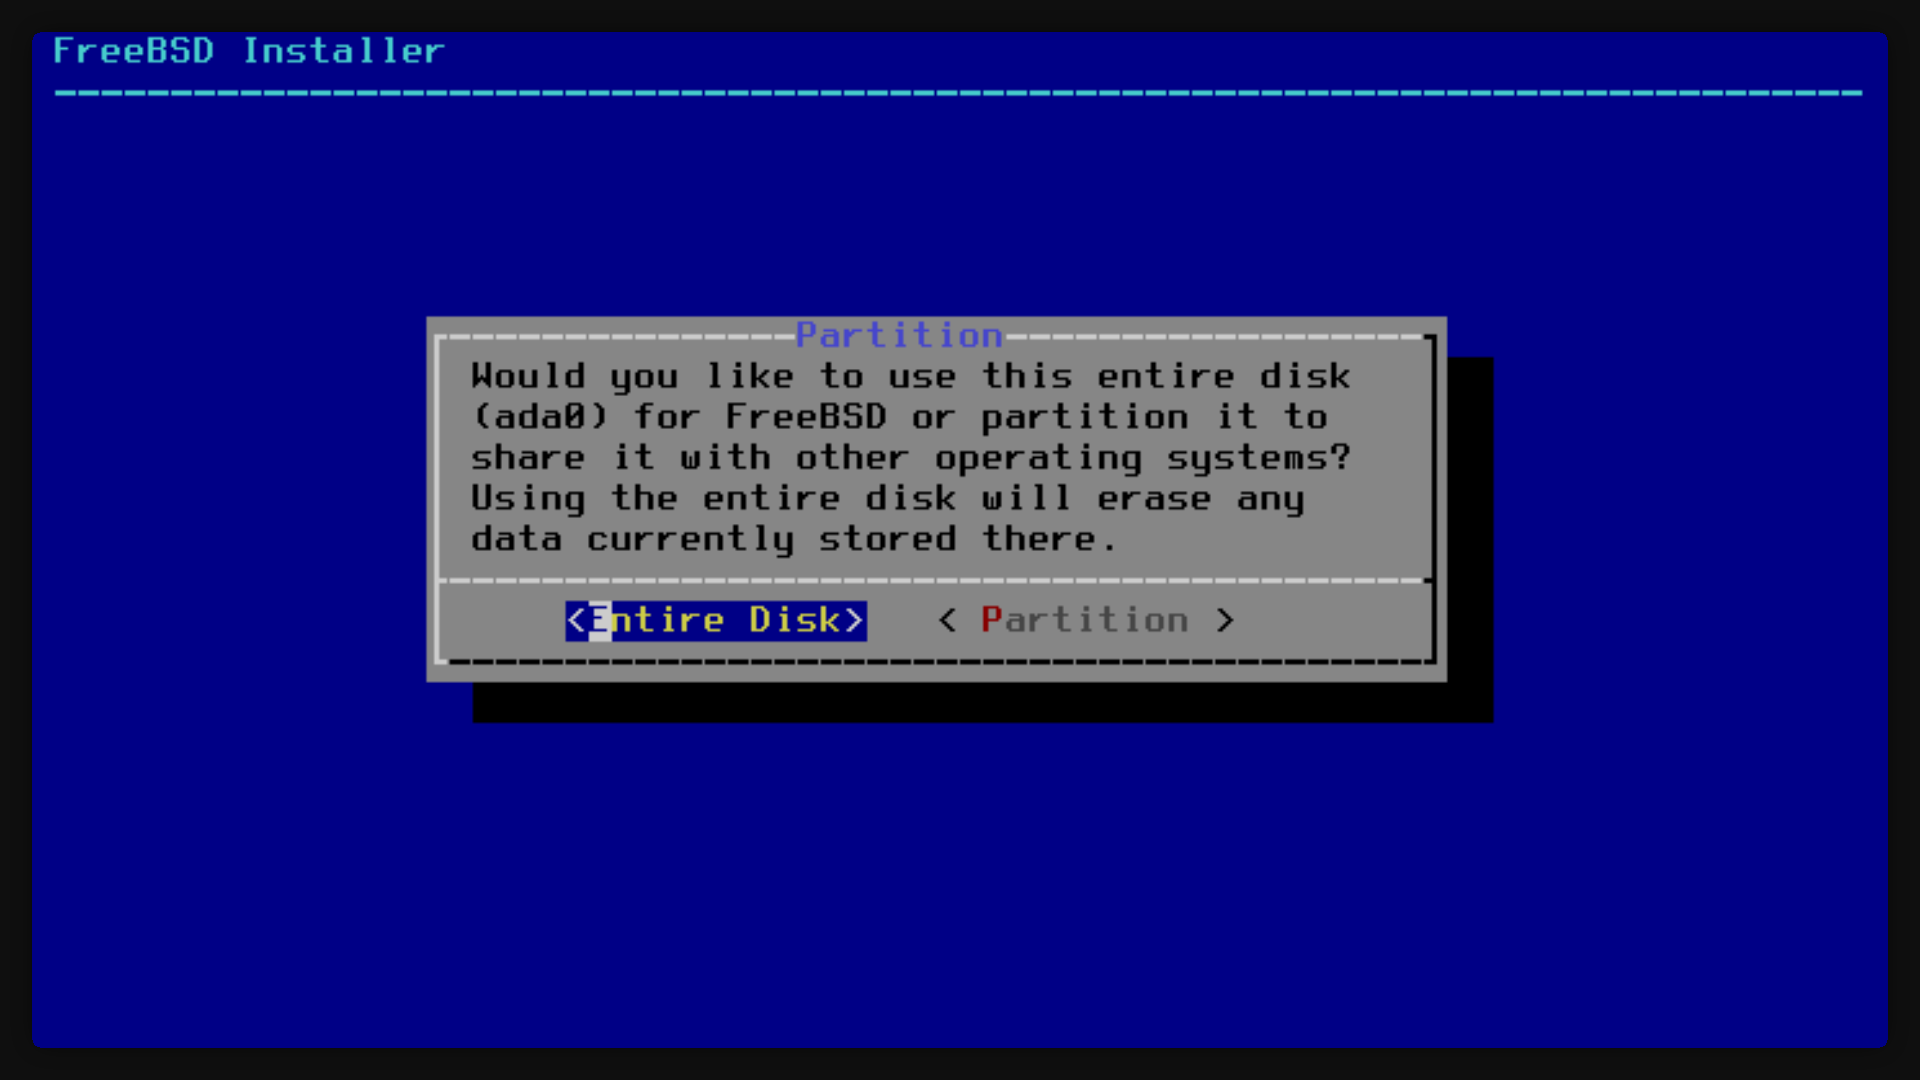
\includegraphics[width=\textwidth,clip=true]{img/8.png}
			\caption{Выделяем весь диск под систему}
		\end{figure}

		\begin{figure}[H]
			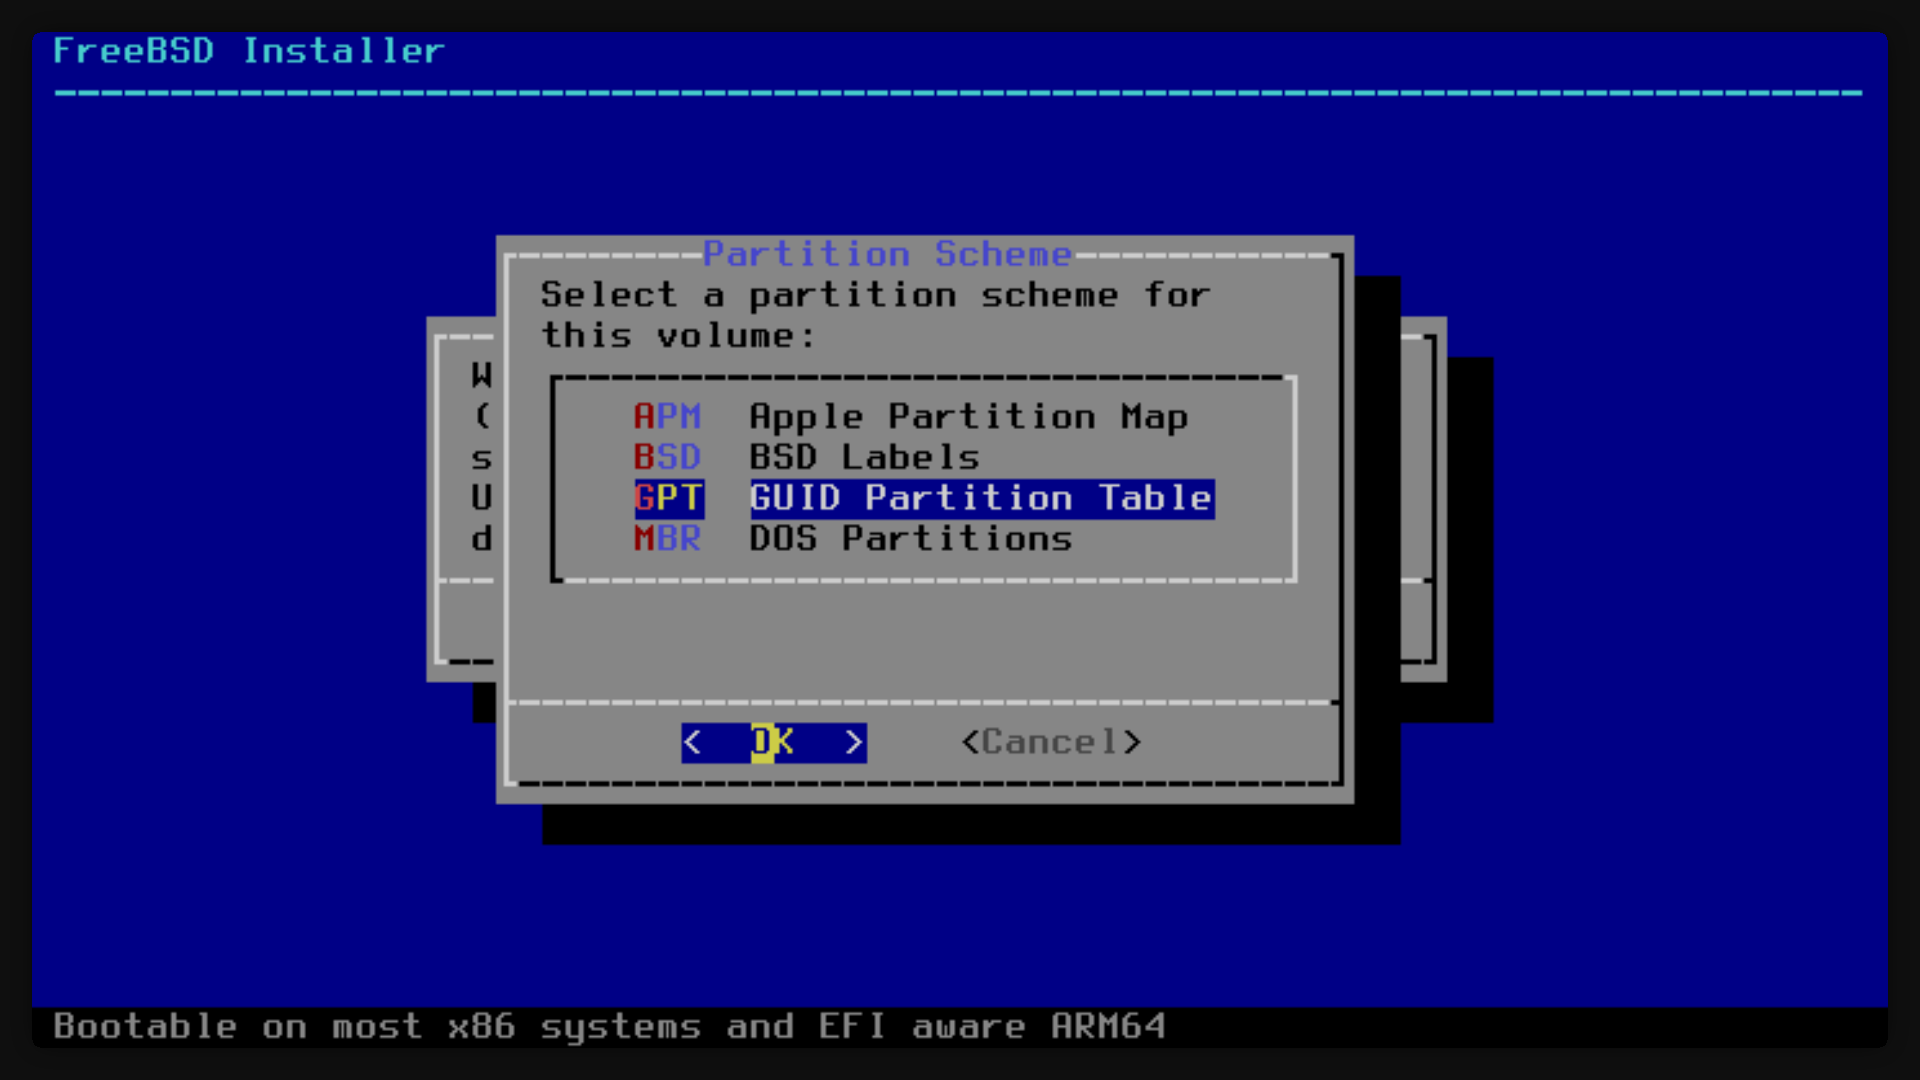
\includegraphics[width=\textwidth,clip=true]{img/9.png}
			\caption{Выбираем таблицу разделов GPT}
		\end{figure}

		\begin{figure}[H]
			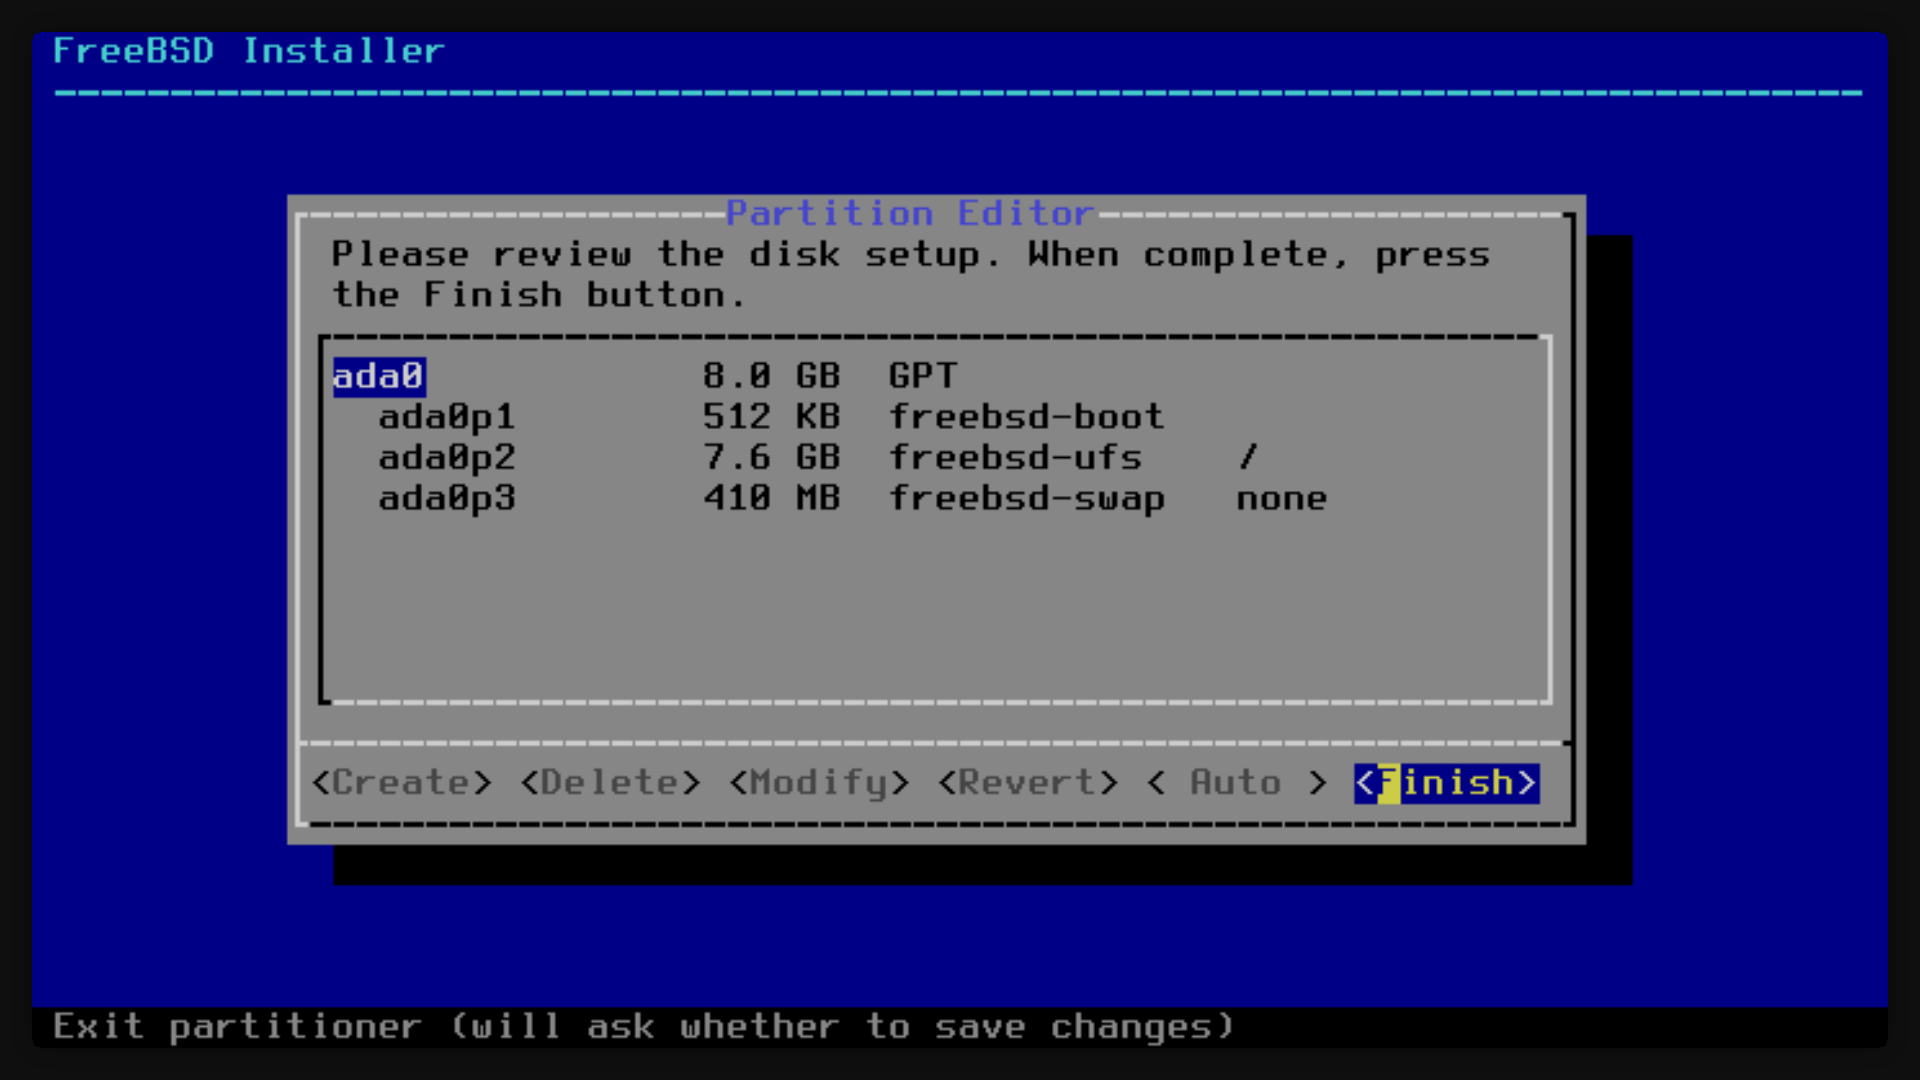
\includegraphics[width=\textwidth,clip=true]{img/10.png}
			\caption{Проверяем, все ли нас устраивает в схеме разметки диска}
		\end{figure}

		\begin{figure}[H]
			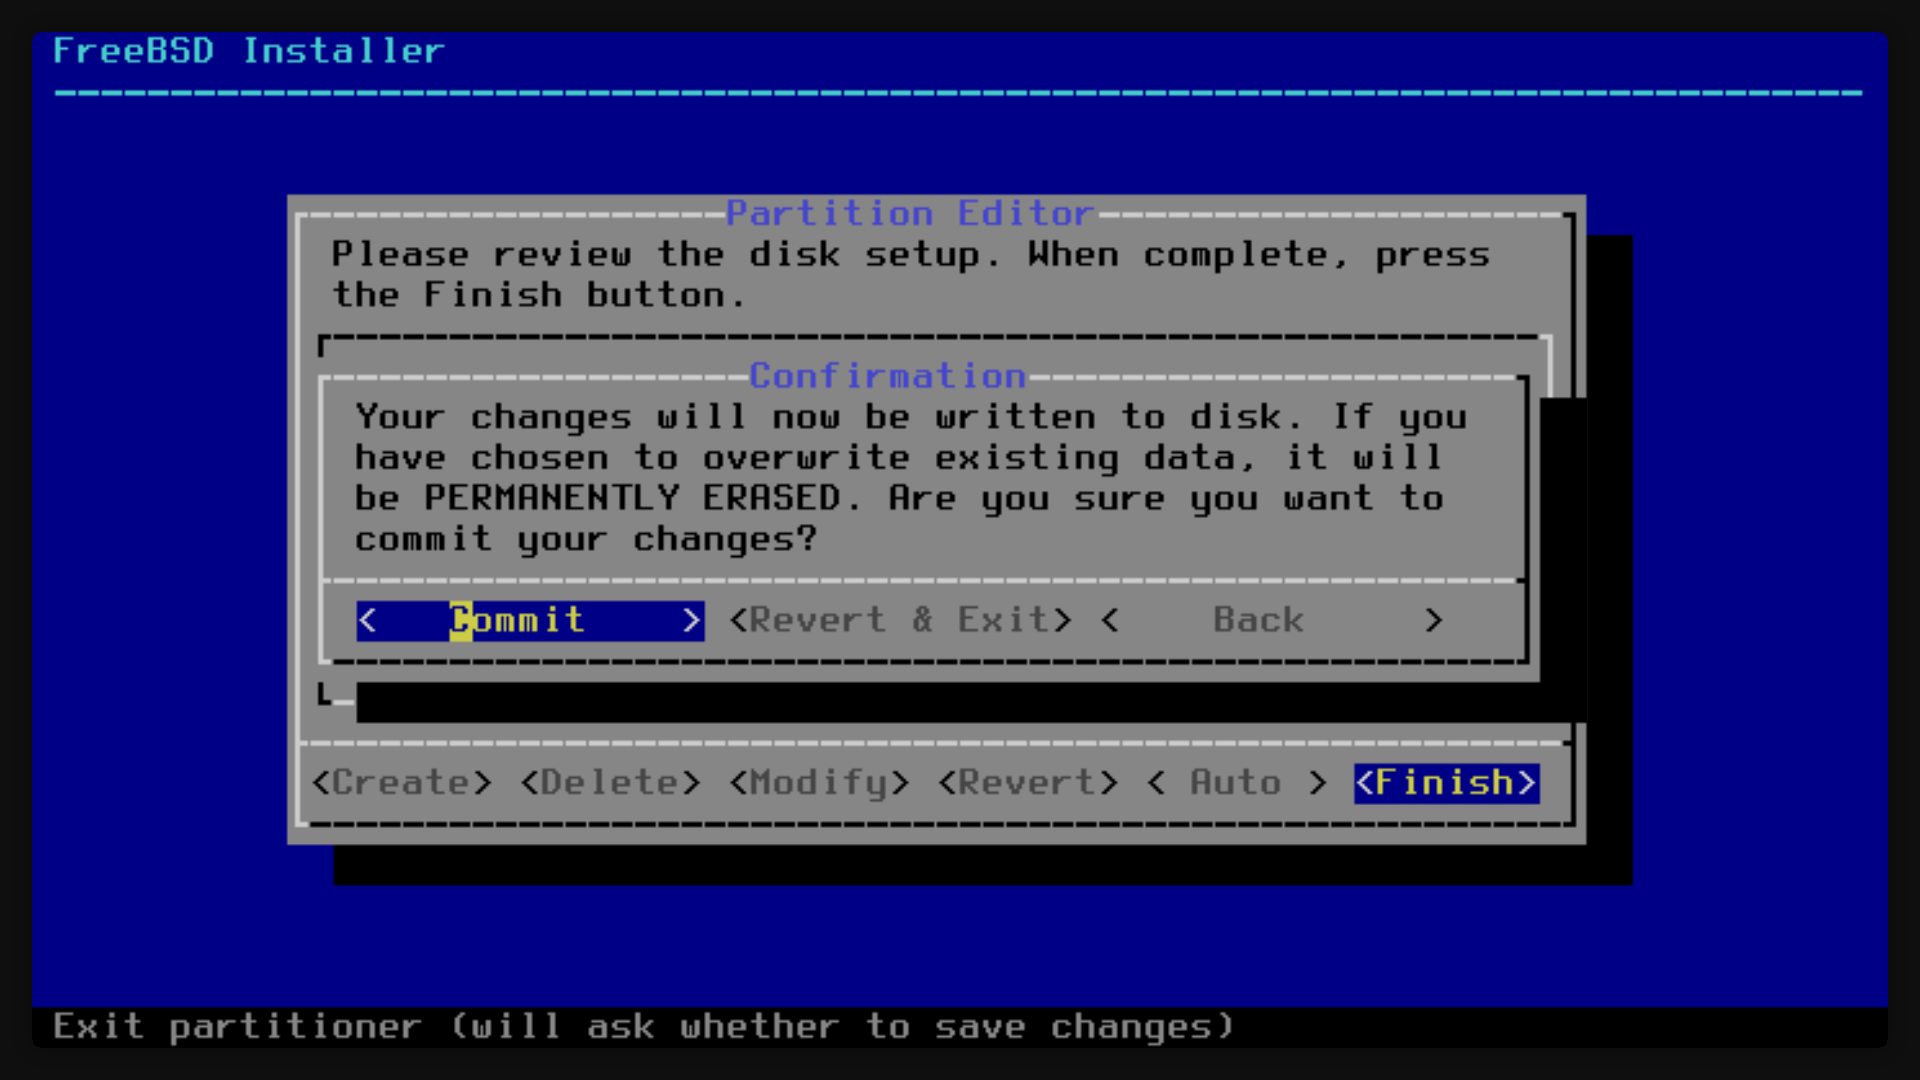
\includegraphics[width=\textwidth,clip=true]{img/11.png}
			\caption{Подтверждаем изменения}
		\end{figure}

	\section{Установка пароля}
		\begin{figure}[H]
			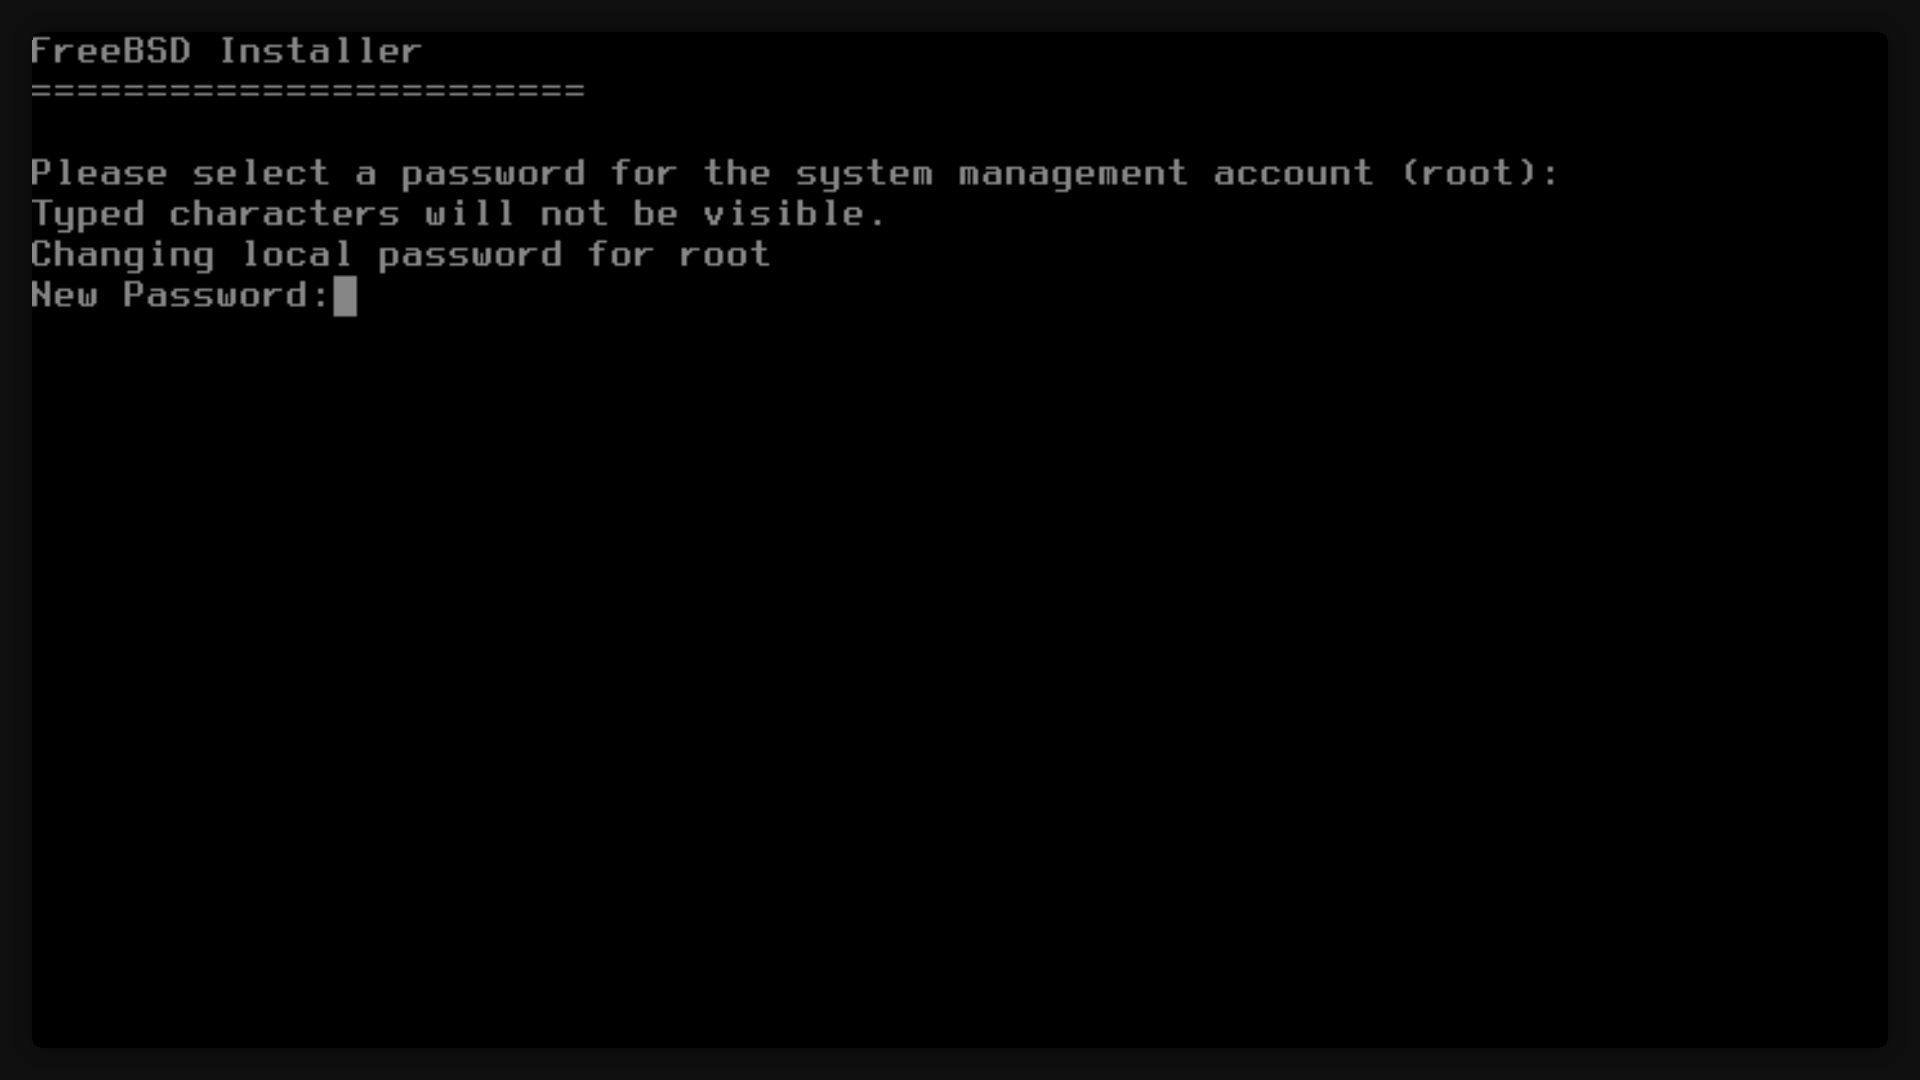
\includegraphics[width=\textwidth,clip=true]{img/12.png}
			\caption{Устанавливаем пароль для пользователя root}
		\end{figure}

	\section{Выбираем часовой пояс}
		\begin{figure}[H]
			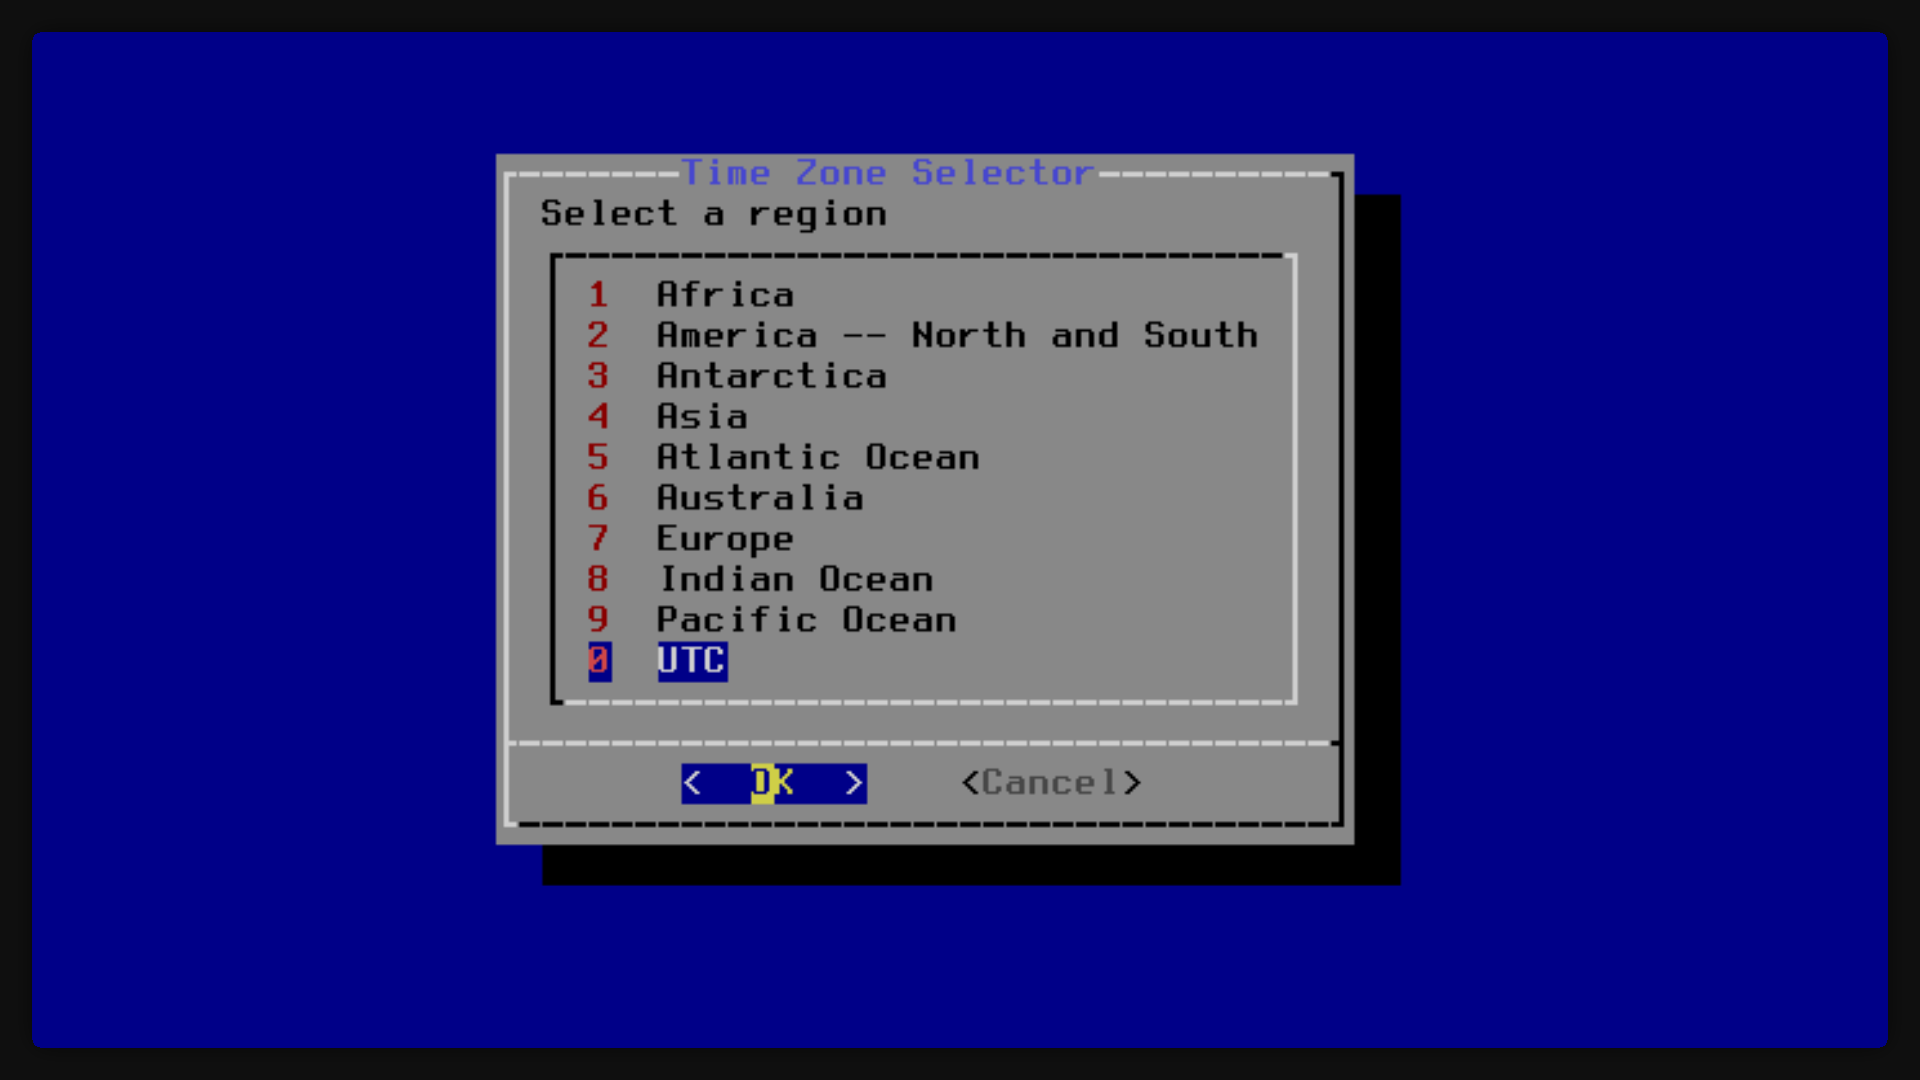
\includegraphics[width=\textwidth,clip=true]{img/13.png}
			\caption{В качестве часового пояса выбираем UTC}
		\end{figure}

	\section{Настройка времени}
		\begin{figure}[H]
			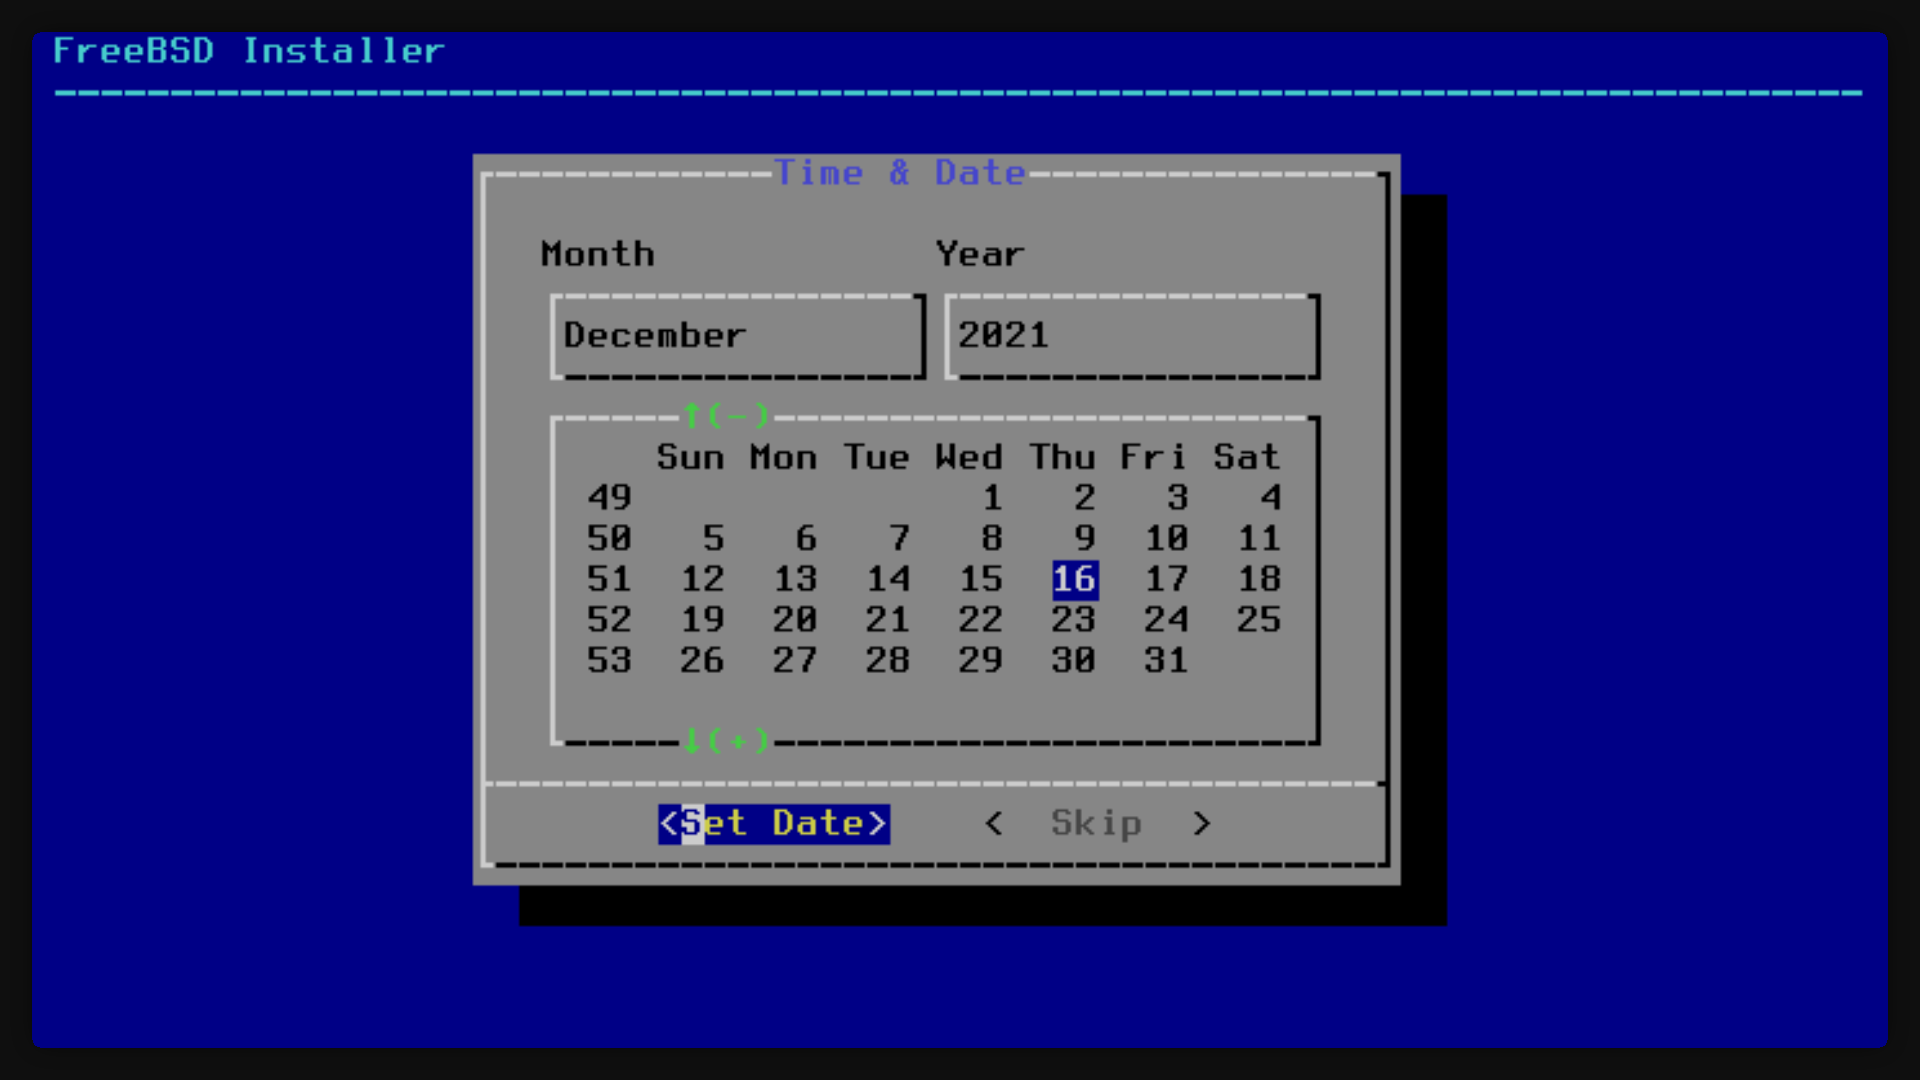
\includegraphics[width=\textwidth,clip=true]{img/14.png}
			\caption{Устанавливаем текущее время}
		\end{figure}

	\section{Настройки безопаности}
		\begin{figure}[H]
			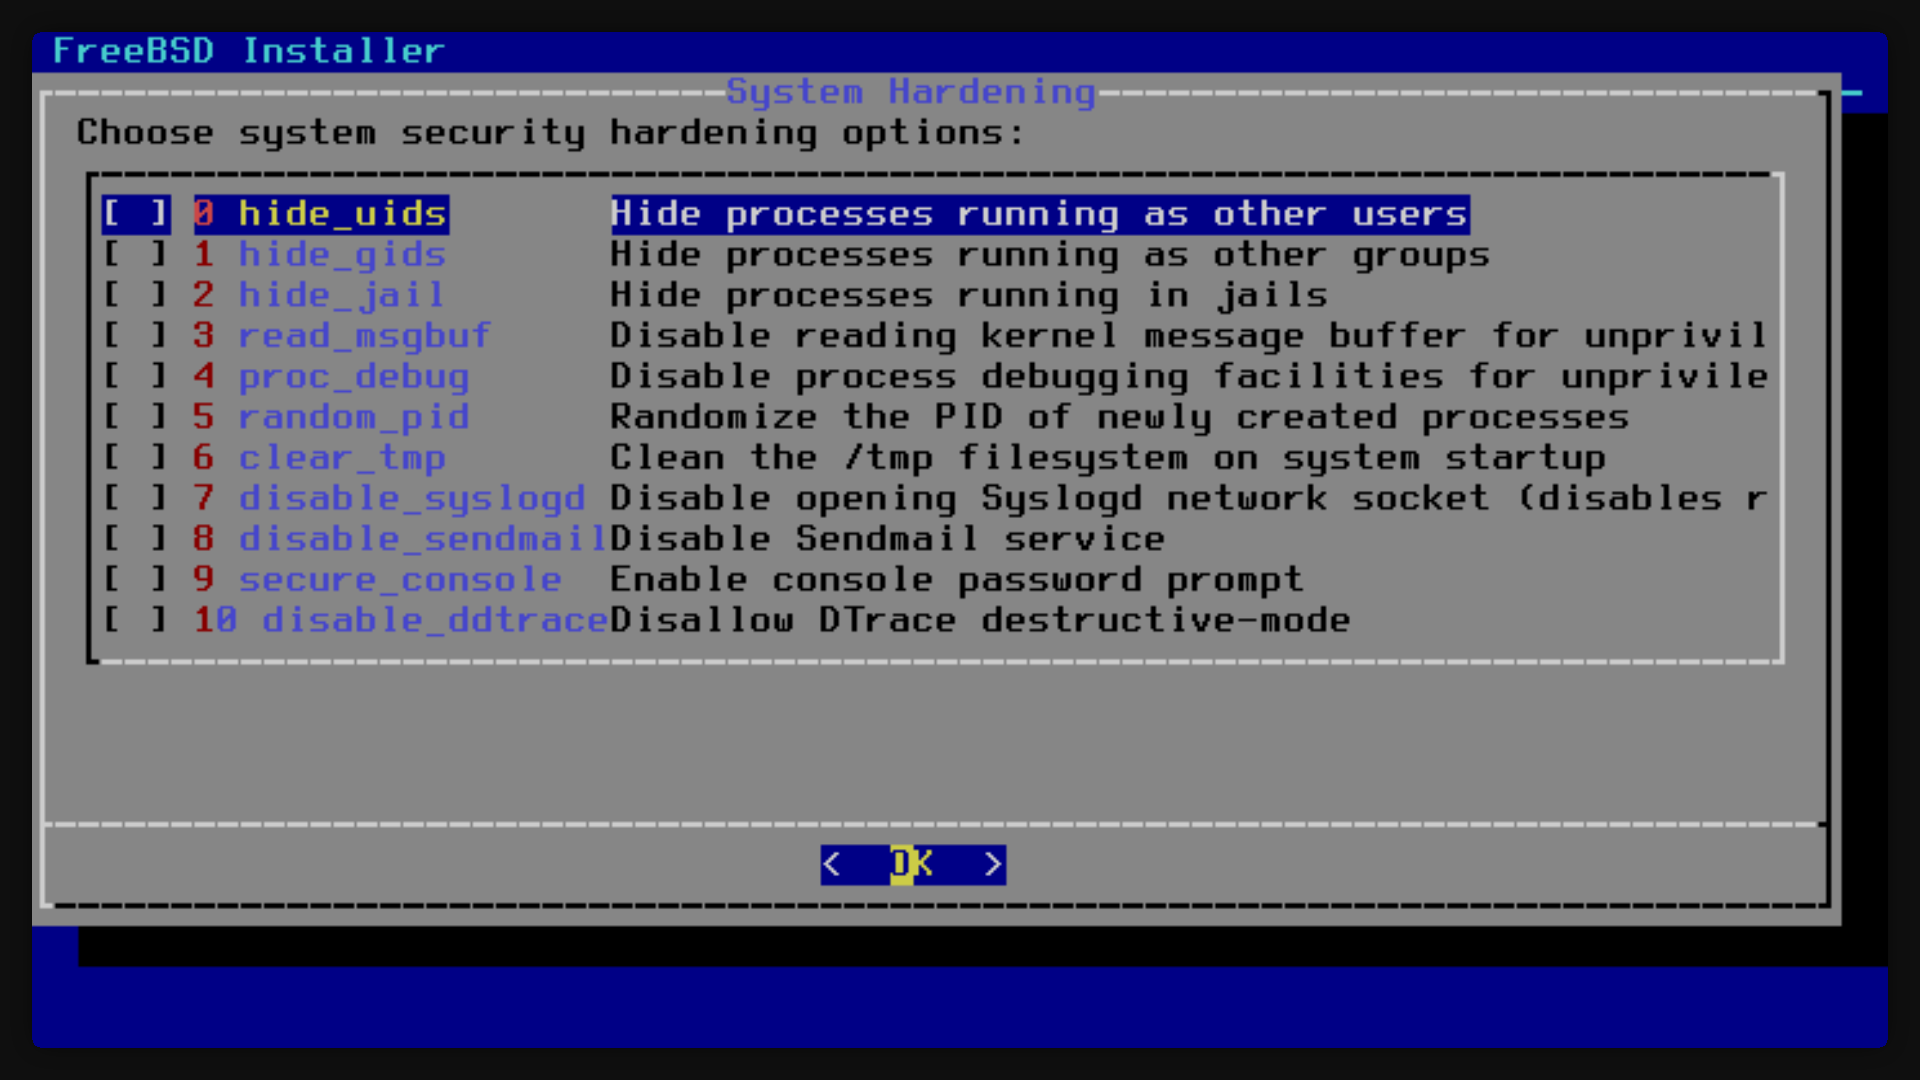
\includegraphics[width=\textwidth,clip=true]{img/15.png}
			\caption{Настройки безопасности оставляем по-умолчанию}
		\end{figure}

	\section{Завершаем установку}
		\begin{figure}[H]
			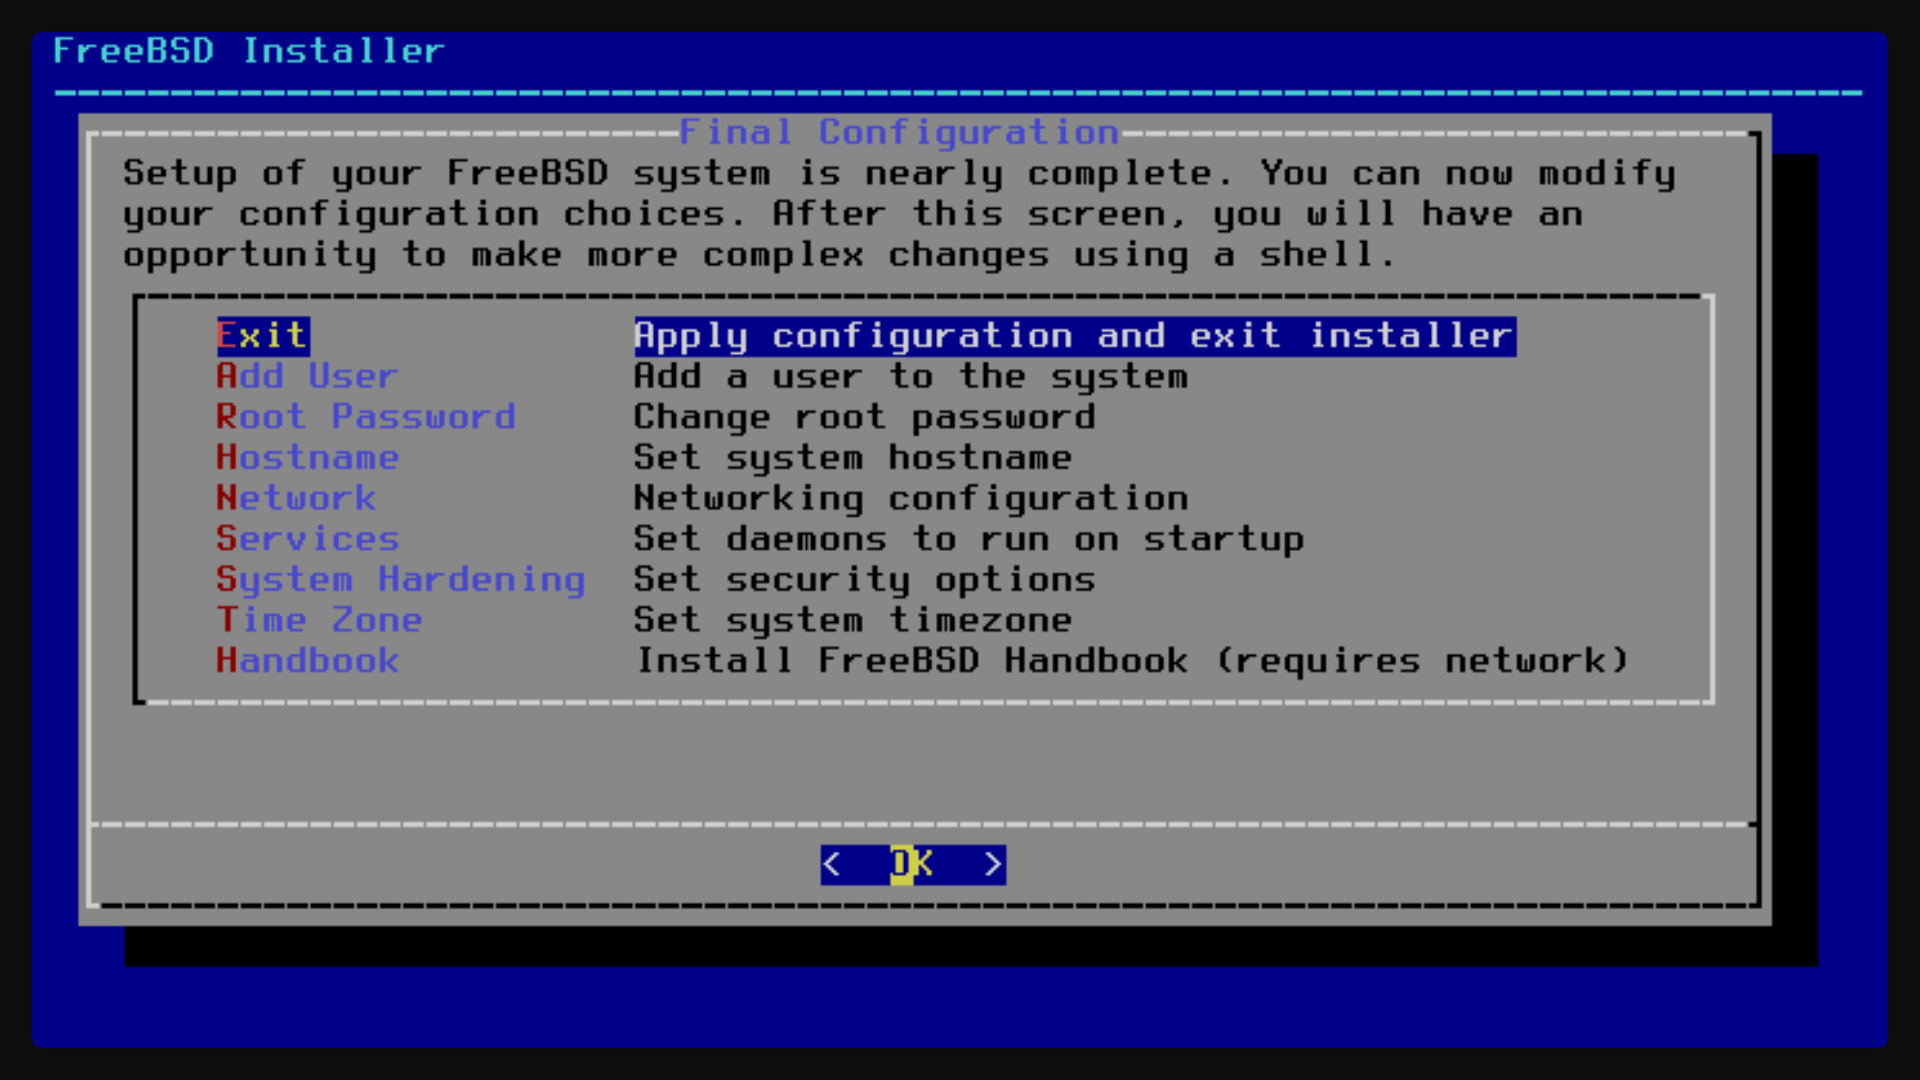
\includegraphics[width=\textwidth,clip=true]{img/16.png}
			\caption{Завершаем установку и перезагружаемся}
		\end{figure}

	\section{Входим в систему}
		\begin{figure}[H]
			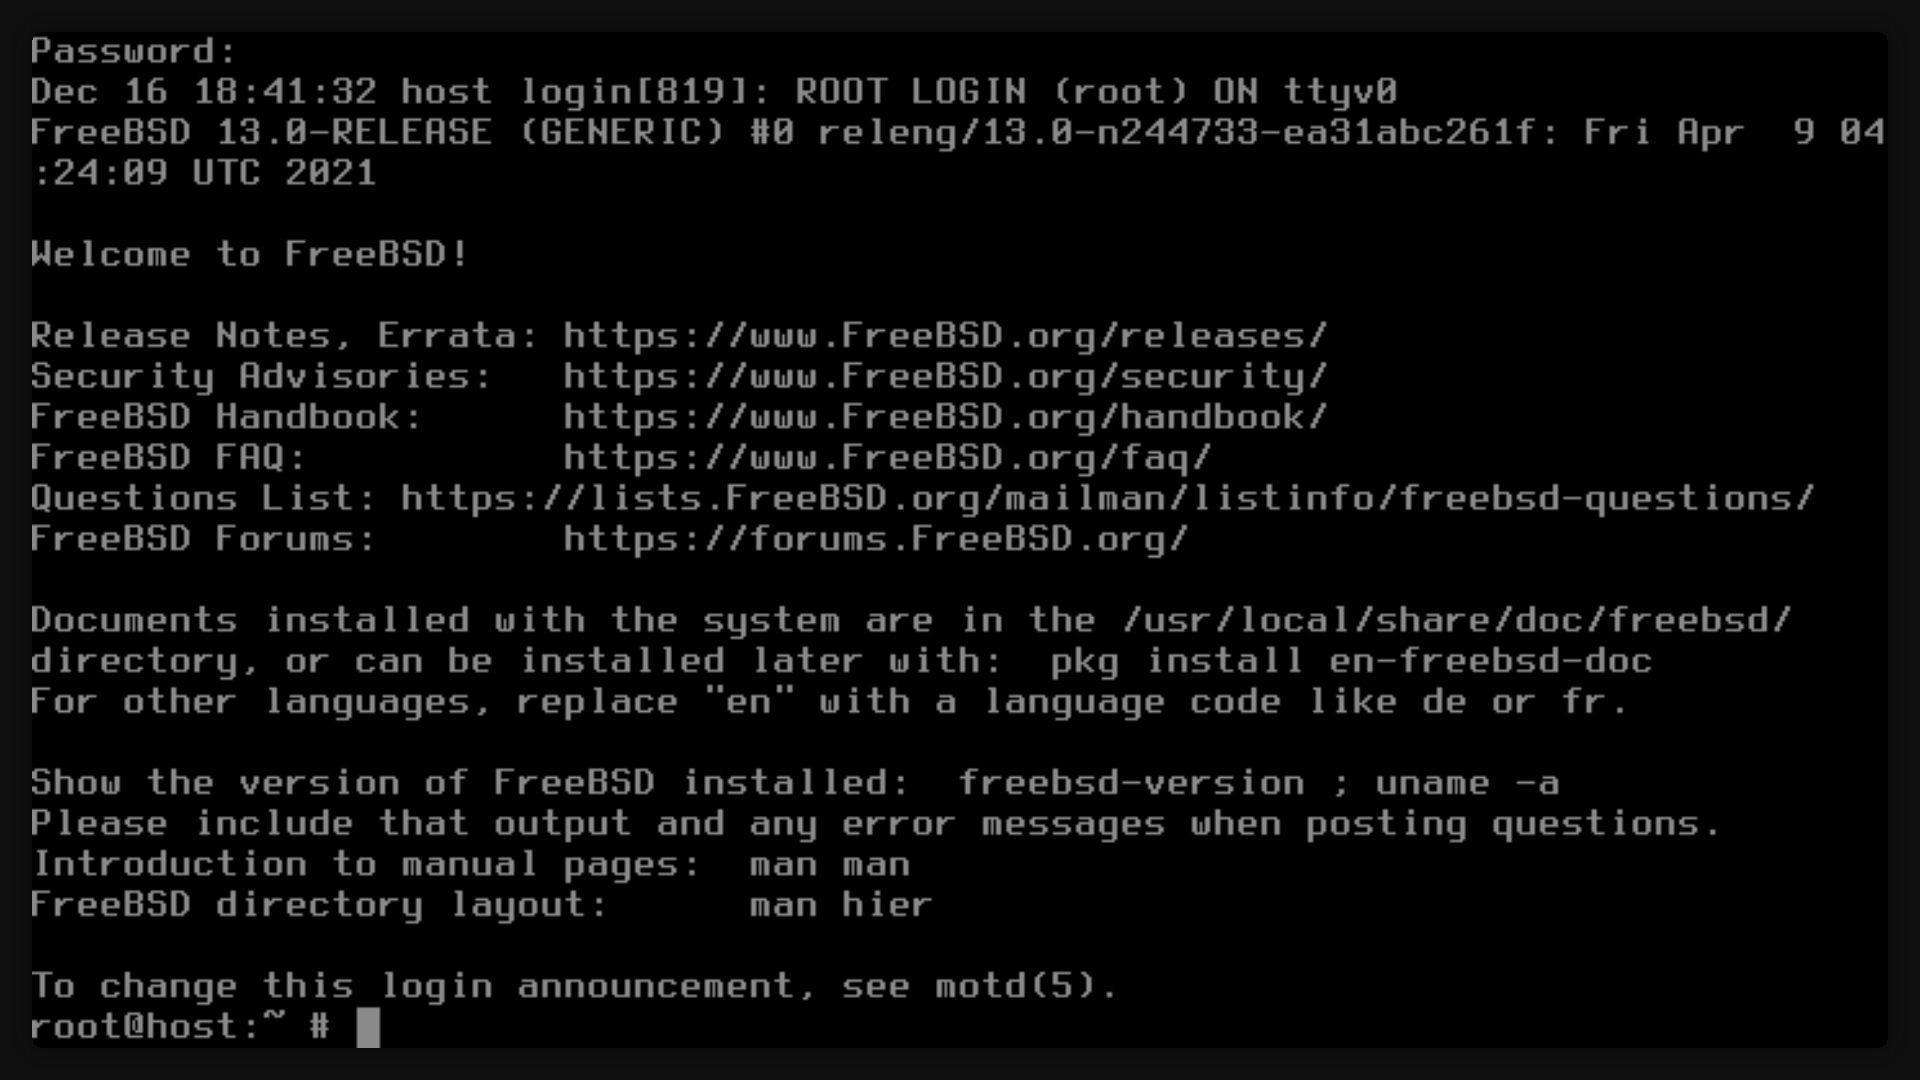
\includegraphics[width=\textwidth,clip=true]{img/17.png}
			\caption{Получаем доступ к командной оболочке свежеустановленной системы}
		\end{figure}
\end{document}
